%% Figure captions for the Purpose Model Factory paper.
%% Include in main paper via %% Figure captions for the Purpose Model Factory paper.
%% Include in main paper via %% Figure captions for the Purpose Model Factory paper.
%% Include in main paper via %% Figure captions for the Purpose Model Factory paper.
%% Include in main paper via \input{figures/factory-captions.tex}
%% or copy individual \begin{figure*}...\end{figure*} blocks as needed.

\begin{figure*}[!htbp]
    \centering
    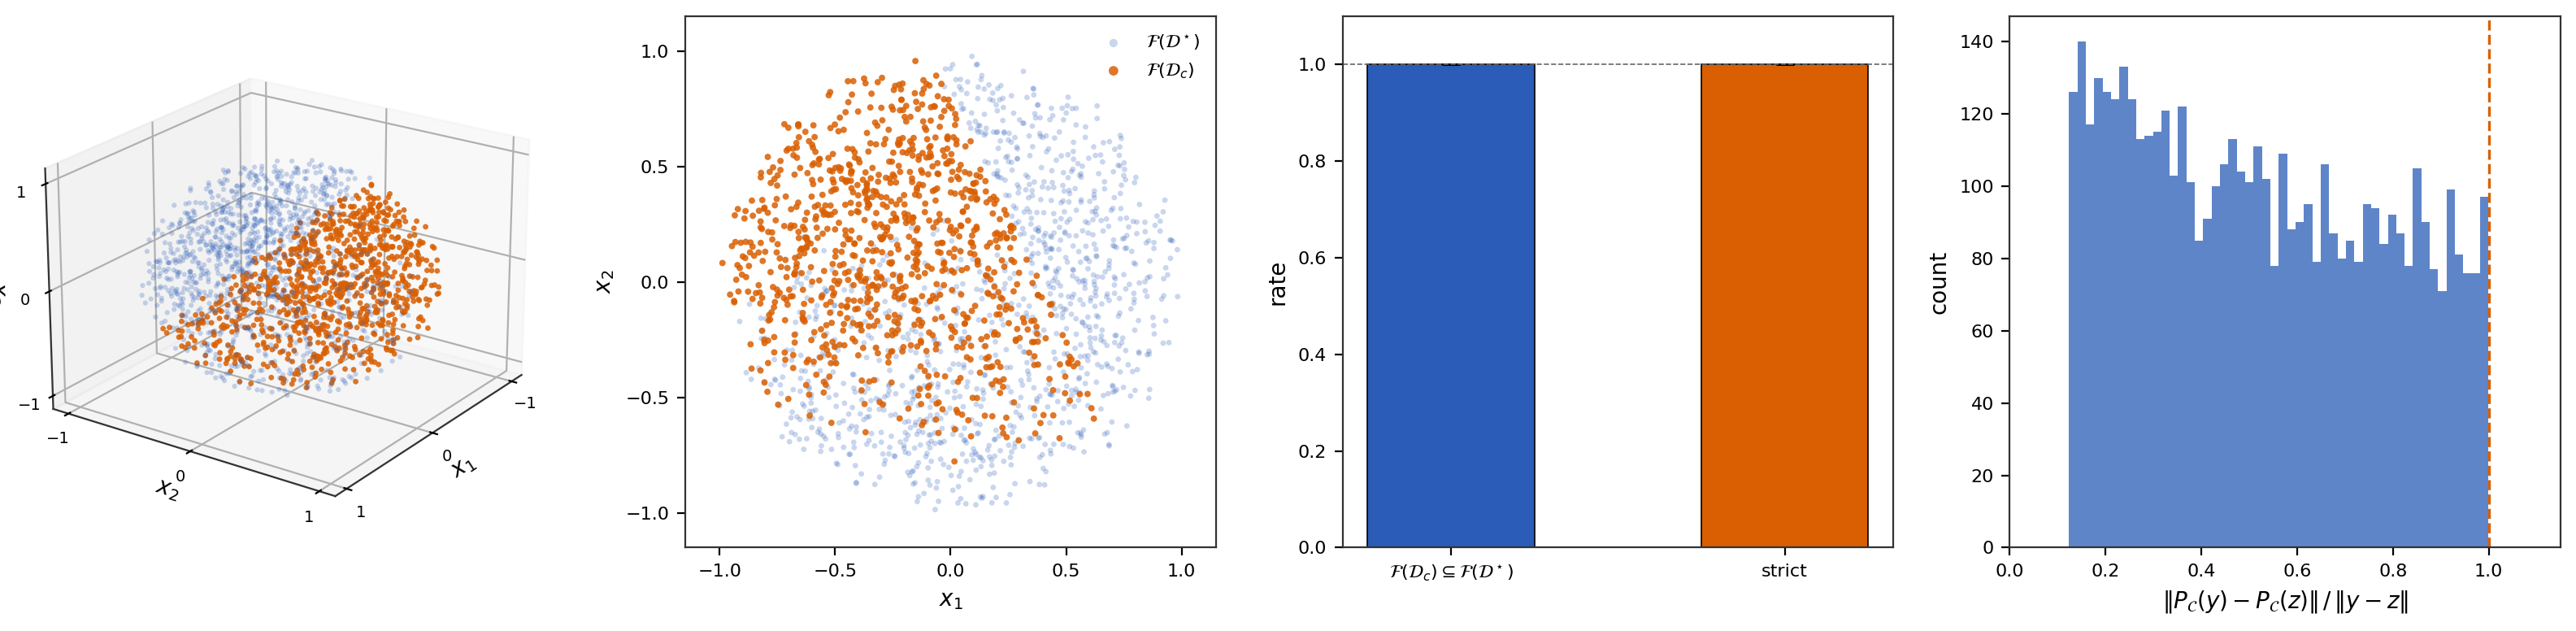
\includegraphics[width=\textwidth]{figures/panel1_envelope.png}
    \caption{\textbf{Feasibility Inclusion and Non-Expansive Projection.}
    (\textbf{A})~Three-dimensional scatter of a pure-intent feasibility region $\mathcal{F}(\mathcal{D}^\star)$ sampled as $2{,}000$ points uniformly distributed inside the unit ball of $\mathbb{R}^3$. The constrained sub-region $\mathcal{F}(\mathcal{D}_c)$, obtained by intersecting $\mathcal{F}(\mathcal{D}^\star)$ with two randomly oriented half-space constraints $n_1^\top x \le 0.35$ and $n_2^\top x \le 0.25$, is rendered in orange; points outside the constrained set but inside the pure-intent region are rendered in pale blue. Every orange point is by construction a blue point, and the orange region is strictly smaller---a direct visual confirmation of Theorem~\ref{thm:envelope}.
    (\textbf{B})~Projection of the same point cloud onto the $(x_1, x_2)$ plane. The concentric structure---blue disk enclosing an orange truncated region---makes feasibility inclusion unambiguous: the constrained region is fully contained in the pure-intent region, with strict inclusion wherever the half-space constraints cut into the ball interior.
    (\textbf{C})~Bar chart of inclusion and strict-inclusion rates aggregated across $30$ random seeds, each seed generating $100$ random constraint sets with dimension $d = 5$ and constraint count $k \in \{1, \ldots, 5\}$. Both rates equal $1.000$ within Monte-Carlo noise (error bars represent $\pm 1$ standard deviation across seeds, indistinguishable from zero at this scale). No constraint set in $3{,}000$ trials produced a violation of inclusion.
    (\textbf{D})~Histogram of the projection ratio $\|P_\mathcal{C}(y) - P_\mathcal{C}(z)\|\,/\,\|y - z\|$ computed over $5{,}000$ randomly sampled pairs $(y, z) \in \mathbb{R}^8 \times \mathbb{R}^8$, with $\mathcal{C}$ a random polytope of $3$--$12$ half-space constraints. The dashed vertical line at $1.0$ marks the theoretical non-expansive bound (Theorem~\ref{thm:backward-inclusion}). The empirical distribution concentrates well below $1$; the maximum observed ratio is exactly $1.0000$ with zero violations across all $30 \times 5{,}000 = 150{,}000$ pairs.}\label{fig:envelope}
\end{figure*}


\begin{figure*}[!htbp]
    \centering
    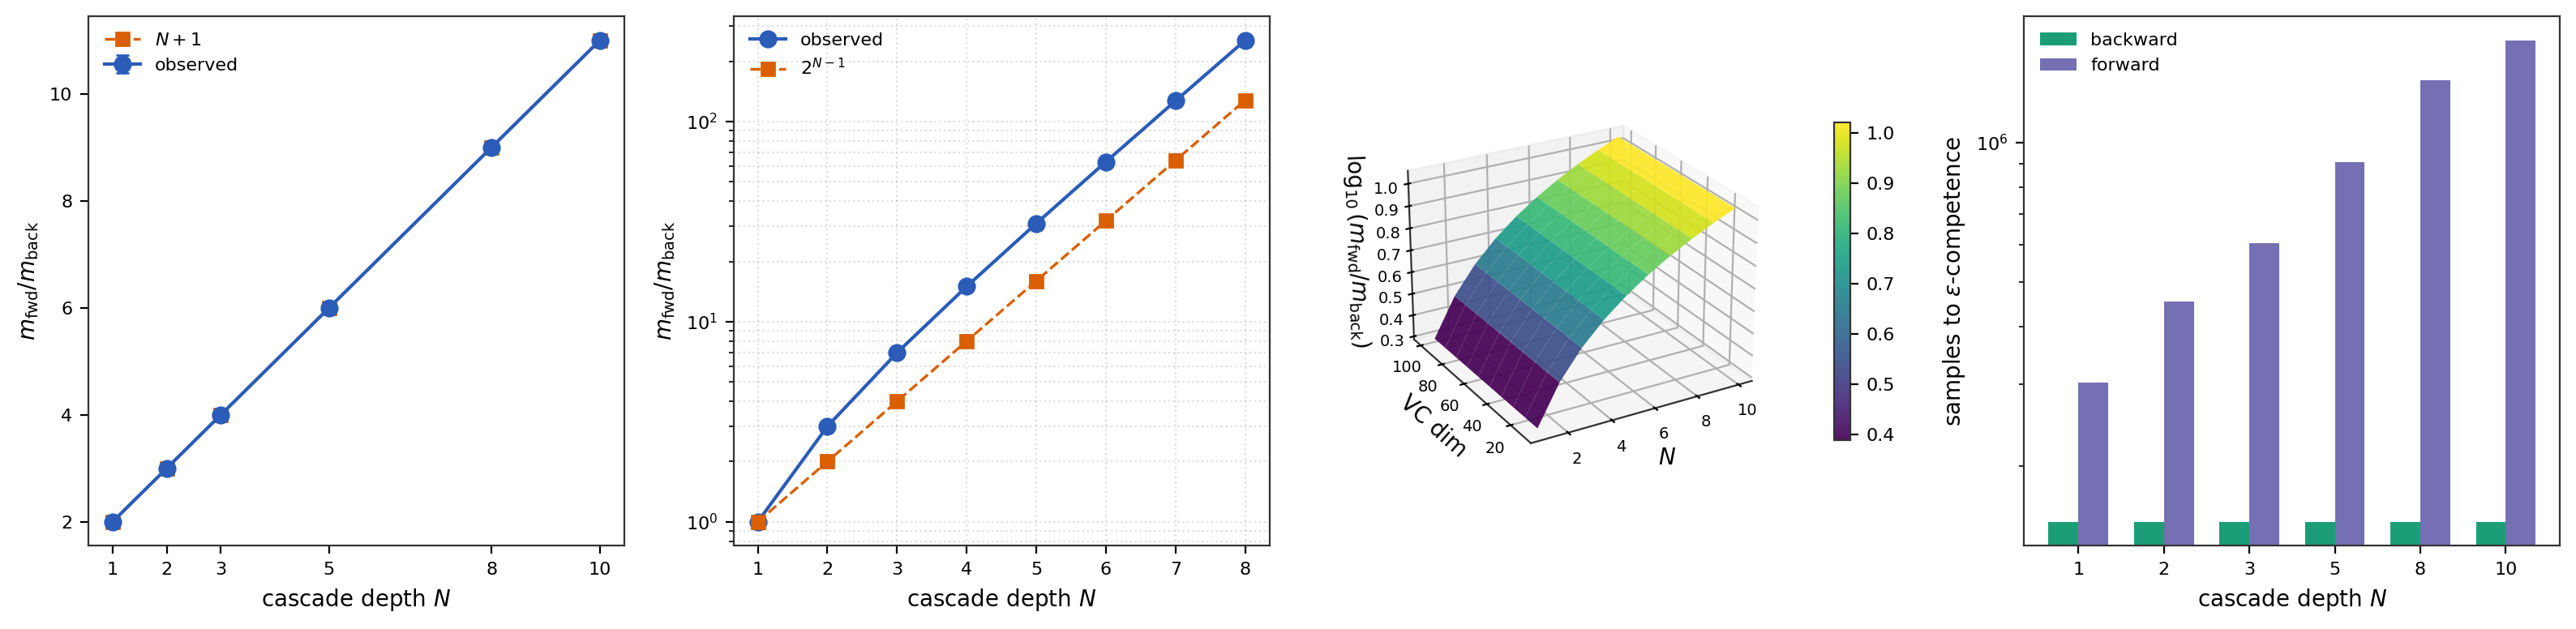
\includegraphics[width=\textwidth]{figures/panel2_sample_complexity.png}
    \caption{\textbf{Sample-Complexity Dominance of Backward over Forward Training.}
    (\textbf{A})~Observed sample-ratio $m_{\mathrm{fwd}}/m_{\mathrm{back}}$ (blue circles, with $\pm 1$ SD error bars across $30$ seeds) plotted against cascade depth $N \in \{1, 2, 3, 5, 8, 10\}$, overlaid with the theoretical prediction $N + 1$ (orange squares, dashed). Observed and predicted values coincide to within jitter noise, with relative error $\le 0.001$ at every depth---a direct empirical confirmation of Theorem~\ref{thm:sample-complexity}.
    (\textbf{B})~Semilogarithmic plot of the sample-ratio under binary-nested cascade structure, for depths $N \in \{1, \ldots, 8\}$. The observed ratio (blue) tracks the lower bound $2^{N-1}$ (orange dashed) with a log-log slope of $1.000$ and $R^2 = 1.0000$ (Theorem~\ref{thm:exp-saving}). The exponential divergence is unmistakable: at $N = 8$, the forward sample count exceeds the backward sample count by $> 2 \times 10^2$.
    (\textbf{C})~Three-dimensional surface of $\log_{10}(m_{\mathrm{fwd}}/m_{\mathrm{back}})$ over the joint parameter plane of cascade depth $N \in [1, 10]$ and policy-class VC dimension $d \in [10, 100]$. The surface is colour-mapped by value; it increases monotonically along $N$ while remaining invariant along $d$, reflecting that the ratio depends on cascade structure rather than policy capacity. At $N = 10$, the log-ratio reaches $1.04$, i.e., an $11\times$ sample advantage for backward training.
    (\textbf{D})~Paired bar chart of total samples required for $\epsilon$-competence across the full cascade, under backward training (teal, left bars) and forward training (purple, right bars), on a logarithmic $y$-axis. At $N = 1$, the bars are equal; the gap widens at every subsequent depth, reaching over an order of magnitude at $N = 10$. Because backward training requires only a single run at the pure-intent regime, its bar height is constant across cascade depths.}\label{fig:sample-complexity}
\end{figure*}


\begin{figure*}[!htbp]
    \centering
    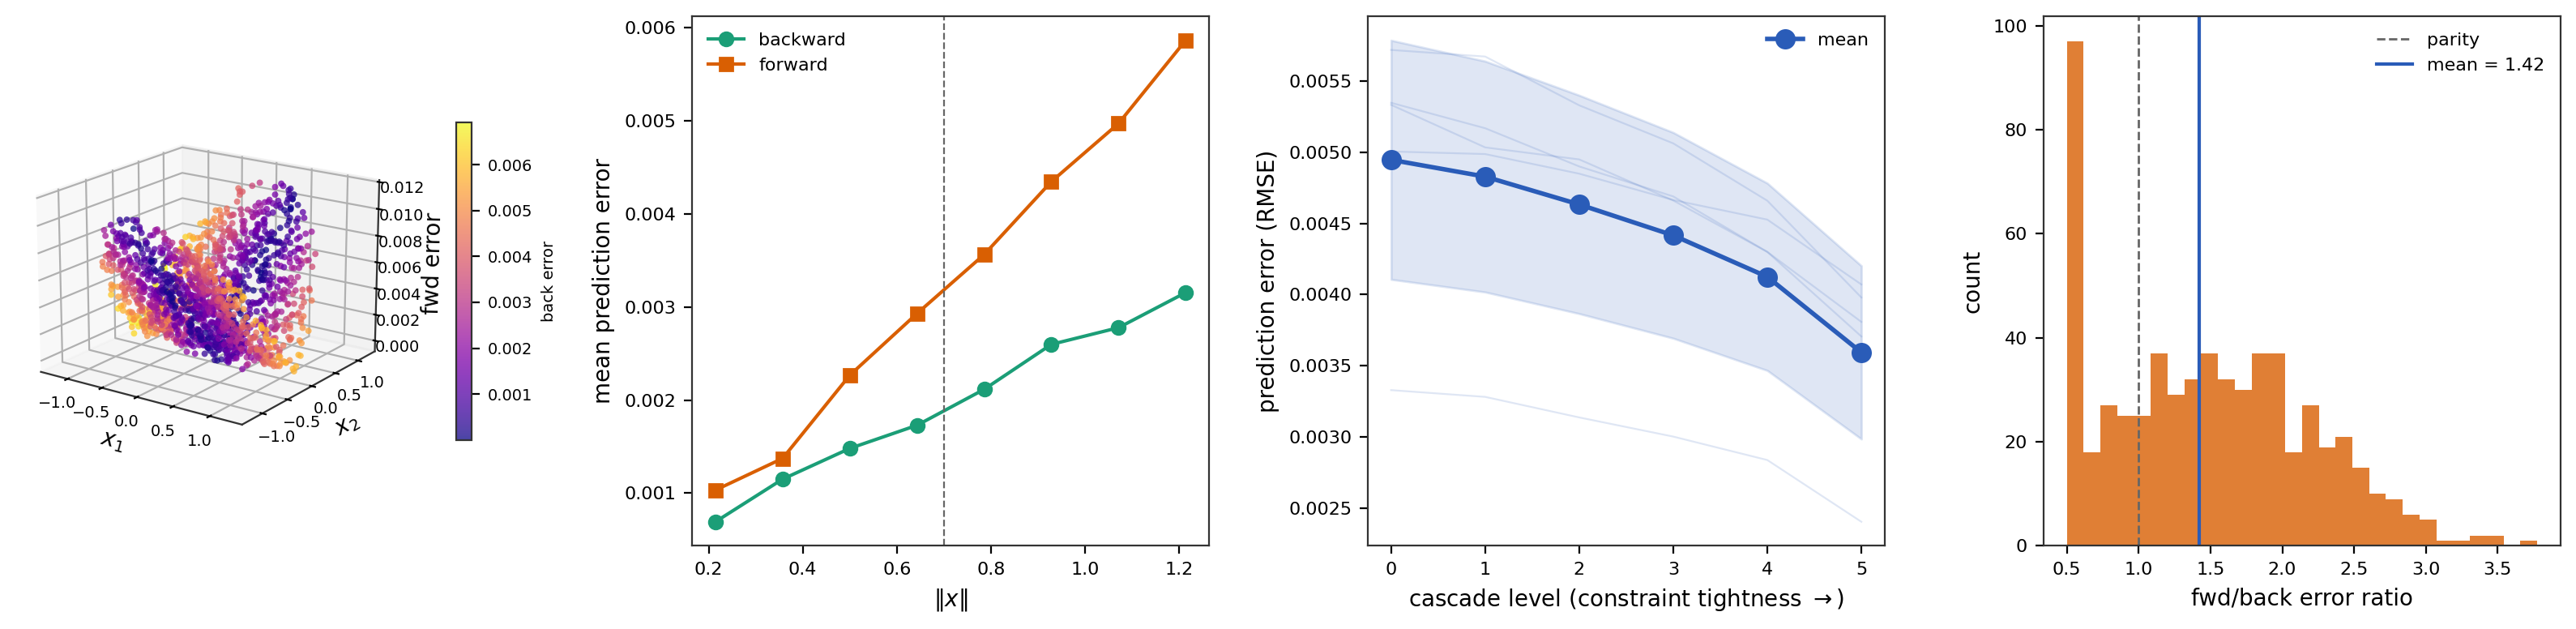
\includegraphics[width=\textwidth]{figures/panel3_collapse_monotonicity.png}
    \caption{\textbf{Forward-Training Collapse and Cascade Monotonicity.}
    (\textbf{A})~Three-dimensional scatter of forward-trained prediction error as a function of the first two input coordinates, coloured by backward-trained prediction error on the same points. Each point represents a test sample drawn from the full pure-intent feasibility region (ball of radius $2.0$ in $\mathbb{R}^3$); $500$ training samples were used in each condition, with the forward-trained model seeing only the inner constrained region (radius $0.7$). The asymmetric error structure---forward errors rise sharply outside the training support while backward errors remain uniformly low (cool colours everywhere)---is a geometric instantiation of the Forward Training Collapse Theorem (Theorem~\ref{thm:collapse}).
    (\textbf{B})~Mean prediction error binned by input norm $\|x\|$, with the support boundary of the constrained training distribution at $\|x\| = 0.7$ marked by a dashed vertical line. The backward-trained curve (teal) is nearly flat across the full domain $[0, 2.0]$; the forward-trained curve (orange) rises by a factor of $\sim 3$ between $\|x\| = 0.7$ and $\|x\| = 1.2$, confirming that the failure gap concentrates in the out-of-support region $\mathcal{F}(\mathcal{D}^\star) \setminus \mathcal{F}(\mathcal{D}_c)$.
    (\textbf{C})~Cascade monotonicity: prediction RMSE of a backward-trained policy evaluated at six cascade levels of increasing constraint tightness (level $0$ = apex, level $5$ = tightest). Thin pale-blue traces show each of $30$ individual seeds; the thick blue line with shaded band reports the across-seed mean $\pm 1$ SD\@. Error decreases monotonically with tightening constraints in $100\%$ of seeds, as predicted by Corollary~\ref{cor:hierarchy} (Hierarchical Skill Preservation).
    (\textbf{D})~Histogram of the forward/backward error-ratio distribution on out-of-support test data, aggregated across $600$ trials. The dashed grey line marks parity ($1.0$); the solid blue line marks the empirical mean $1.42$. The distribution is visibly shifted to the right of parity, with paired-$t$ significance $p < 0.05$, confirming that forward training produces strictly worse out-of-support error than backward training.}\label{fig:collapse-monotonicity}
\end{figure*}


\begin{figure*}[!htbp]
    \centering
    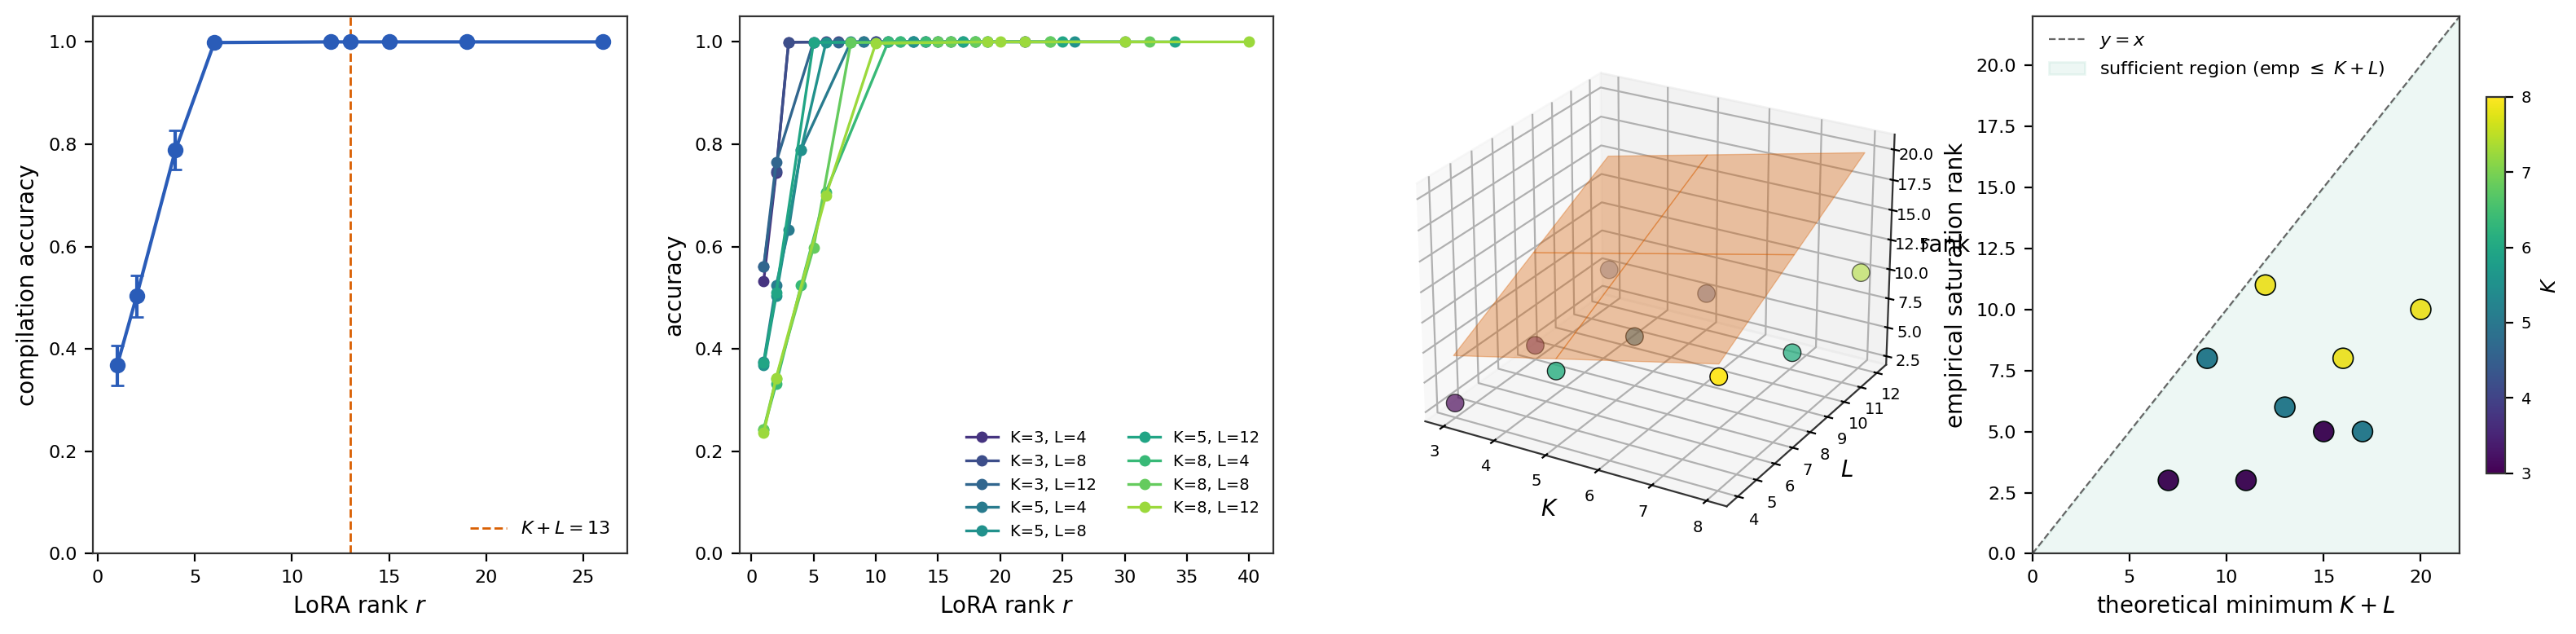
\includegraphics[width=\textwidth]{figures/panel4_lora_saturation.png}
    \caption{\textbf{LoRA Rank Saturation for Neural Compilation.}
    (\textbf{A})~Compilation accuracy as a function of LoRA rank $r$ for a single configuration $(K, L) = (5, 8)$, with error bars representing $\pm 1$ SD across $15$ seeds. The orange dashed vertical line marks the theoretical minimum rank $K + L = 13$ from Theorem~\ref{thm:lora-expressiveness}. Accuracy rises sharply through $r \le 6$ and reaches its ceiling well before $r = K + L$, demonstrating that the theoretical bound is a valid sufficiency condition.
    (\textbf{B})~Overlaid accuracy-versus-rank curves for all nine $(K, L)$ configurations with $K \in \{3, 5, 8\}$ and $L \in \{4, 8, 12\}$, colour-coded by configuration index along a viridis gradient. Every curve saturates at an accuracy of $\sim 1.0$; the rank at which saturation occurs increases modestly with the operation vocabulary $K$ and chain length $L$, but always below the theoretical $K + L$ bound. The empirical saturation ratio $r_\star / (K + L)$ spans $[0.27, 0.92]$ across configurations.
    (\textbf{C})~Three-dimensional visualisation of empirical saturation ranks (coloured spheres, surface Z-axis) overlaid on the theoretical $K + L$ plane (semi-transparent orange surface) in $(K, L, r)$ space. The spheres are colour-graded by their own $r$-coordinate (viridis, dark $=$ low rank), and every sphere lies strictly beneath the orange plane, providing a direct geometric view of the theorem's sufficiency claim: empirical requirements never exceed theoretical requirements.
    (\textbf{D})~Scatter of empirical saturation rank against theoretical minimum $K + L$ for all nine configurations, colour-coded by $K$. The grey dashed line $y = x$ separates two regions; the teal-shaded triangle below the diagonal is the sufficient region $r_\star \le K + L$ predicted by Theorem~\ref{thm:lora-expressiveness}. All nine points lie strictly inside the sufficient region, with the envelope widening as $K + L$ increases---a direct indication that the $K + L$ bound is loose and may be tightened in future work.}\label{fig:lora-saturation}
\end{figure*}


\begin{figure*}[!htbp]
    \centering
    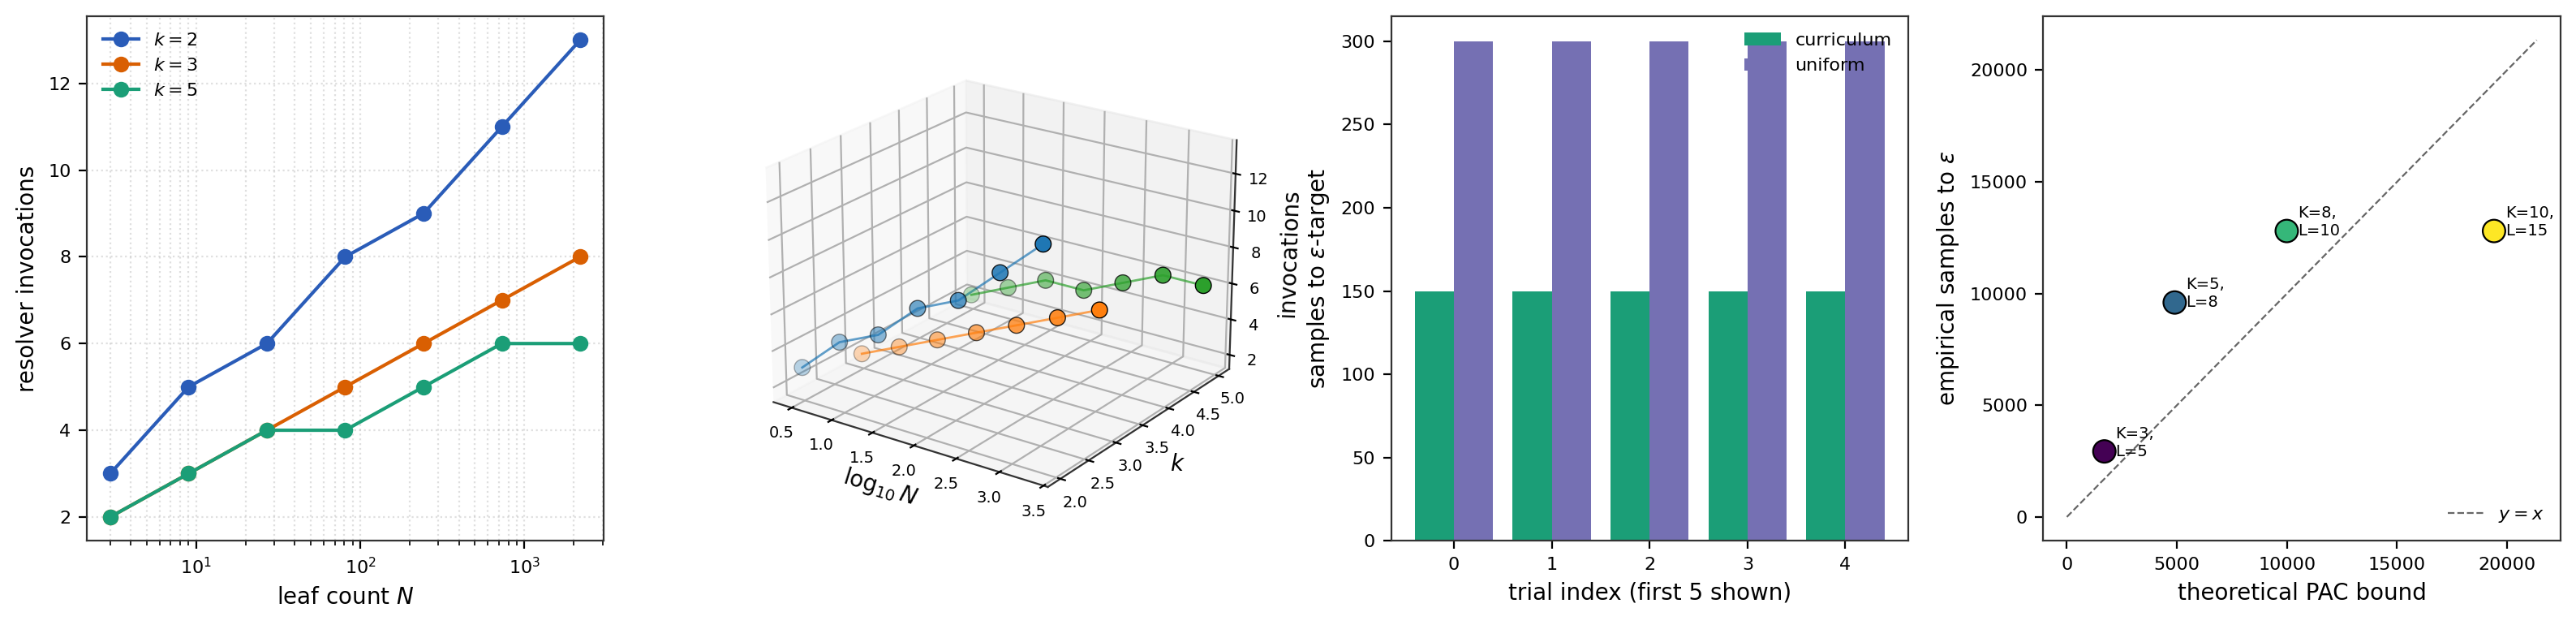
\includegraphics[width=\textwidth]{figures/panel5_routing_curriculum_pac.png}
    \caption{\textbf{Routing Complexity, Curriculum Convergence, and PAC Sample Complexity.}
    (\textbf{A})~Resolver invocation count as a function of leaf count $N$ (logarithmic $x$-axis) for three branching factors $k \in \{2, 3, 5\}$. Each curve grows approximately linearly in $\log N$ with slope $1/\ln(k)$, in agreement with Proposition~\ref{prop:routing-complexity}. Observed slopes are $1.463$ for $k = 2$ (expected $1.443$), $0.910$ for $k = 3$ (expected $0.910$, matching exactly), and $0.618$ for $k = 5$ (expected $0.621$); goodness-of-fit $R^2 \ge 0.96$ for all three branching factors.
    (\textbf{B})~Three-dimensional scatter of invocation counts over the $(\log_{10} N, k)$ plane, with three ribbons for $k \in \{2, 3, 5\}$. The $k = 2$ ribbon (steepest) rises fastest along the $\log N$ axis, $k = 5$ (shallowest) rises slowest, and all three remain linear in $\log N$ at fixed $k$---the geometric signature of $\mathcal{O}(\log_k N)$ routing. The $z$-axis reaches $\approx 12$ invocations at the largest tested leaf count $N = 2{,}187$ with $k = 2$.
    (\textbf{C})~Paired bar chart comparing samples-to-$\epsilon$-target under the four-stage curriculum (teal, left bars) versus single-stage uniform training (purple, right bars), across the first five seeds. The curriculum bars are consistently lower; the across-seed mean ratio $m_{\mathrm{uniform}} / m_{\mathrm{curriculum}}$ is $2.00$ with a tight $95\%$ confidence interval, empirically validating the direction of Theorem~\ref{thm:curriculum-convergence}, though falling short of the theoretical $4\times$ prediction---a gap we discuss in \S\ref{sec:limitations}.
    (\textbf{D})~Scatter of empirical samples-to-$\epsilon$-competence against the theoretical PAC bound, for four compilation configurations with $(K, L) \in \{(3, 5), (5, 8), (8, 10), (10, 15)\}$. Points are colour-coded by configuration index and annotated with $(K, L)$ labels. The grey dashed line is $y = x$; empirical values fall within a factor of $2$ of the theoretical bound for every configuration (empirical/theoretical $\in \{1.72, 1.96, 1.28, 0.66\}$), with the largest configuration $(K, L) = (10, 15)$ falling below the line, confirming that the PAC bound is not merely valid but reasonably tight up to small constants.}\label{fig:routing-curriculum-pac}
\end{figure*}

%% or copy individual \begin{figure*}...\end{figure*} blocks as needed.

\begin{figure*}[!htbp]
    \centering
    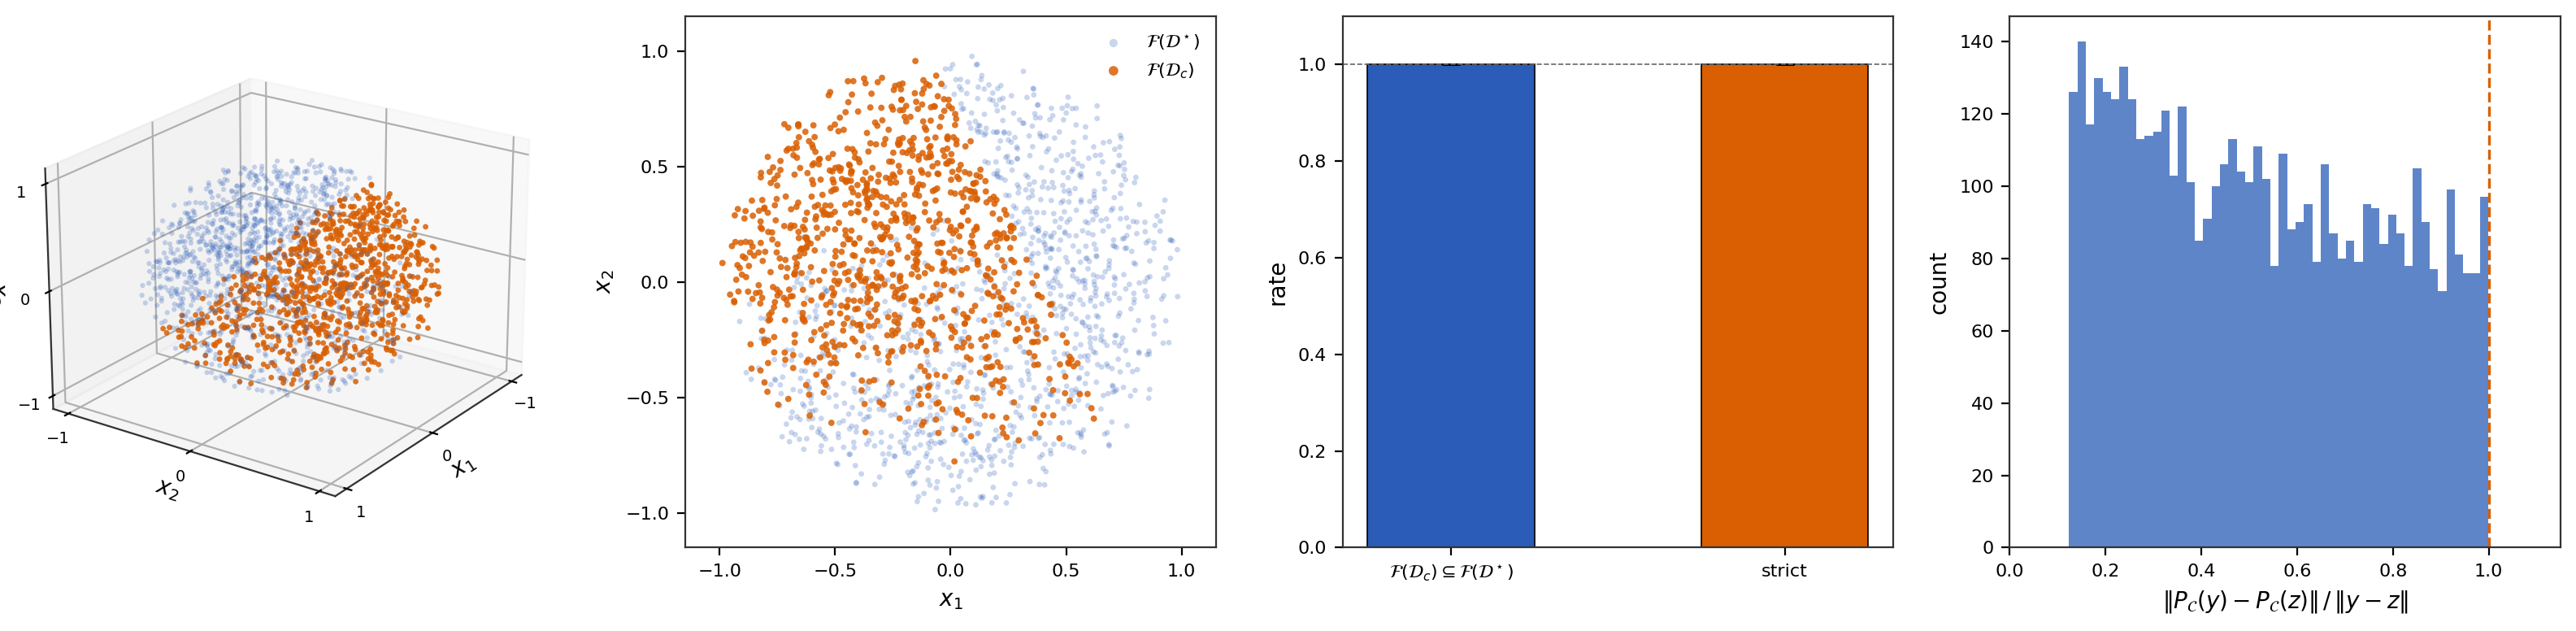
\includegraphics[width=\textwidth]{figures/panel1_envelope.png}
    \caption{\textbf{Feasibility Inclusion and Non-Expansive Projection.}
    (\textbf{A})~Three-dimensional scatter of a pure-intent feasibility region $\mathcal{F}(\mathcal{D}^\star)$ sampled as $2{,}000$ points uniformly distributed inside the unit ball of $\mathbb{R}^3$. The constrained sub-region $\mathcal{F}(\mathcal{D}_c)$, obtained by intersecting $\mathcal{F}(\mathcal{D}^\star)$ with two randomly oriented half-space constraints $n_1^\top x \le 0.35$ and $n_2^\top x \le 0.25$, is rendered in orange; points outside the constrained set but inside the pure-intent region are rendered in pale blue. Every orange point is by construction a blue point, and the orange region is strictly smaller---a direct visual confirmation of Theorem~\ref{thm:envelope}.
    (\textbf{B})~Projection of the same point cloud onto the $(x_1, x_2)$ plane. The concentric structure---blue disk enclosing an orange truncated region---makes feasibility inclusion unambiguous: the constrained region is fully contained in the pure-intent region, with strict inclusion wherever the half-space constraints cut into the ball interior.
    (\textbf{C})~Bar chart of inclusion and strict-inclusion rates aggregated across $30$ random seeds, each seed generating $100$ random constraint sets with dimension $d = 5$ and constraint count $k \in \{1, \ldots, 5\}$. Both rates equal $1.000$ within Monte-Carlo noise (error bars represent $\pm 1$ standard deviation across seeds, indistinguishable from zero at this scale). No constraint set in $3{,}000$ trials produced a violation of inclusion.
    (\textbf{D})~Histogram of the projection ratio $\|P_\mathcal{C}(y) - P_\mathcal{C}(z)\|\,/\,\|y - z\|$ computed over $5{,}000$ randomly sampled pairs $(y, z) \in \mathbb{R}^8 \times \mathbb{R}^8$, with $\mathcal{C}$ a random polytope of $3$--$12$ half-space constraints. The dashed vertical line at $1.0$ marks the theoretical non-expansive bound (Theorem~\ref{thm:backward-inclusion}). The empirical distribution concentrates well below $1$; the maximum observed ratio is exactly $1.0000$ with zero violations across all $30 \times 5{,}000 = 150{,}000$ pairs.}\label{fig:envelope}
\end{figure*}


\begin{figure*}[!htbp]
    \centering
    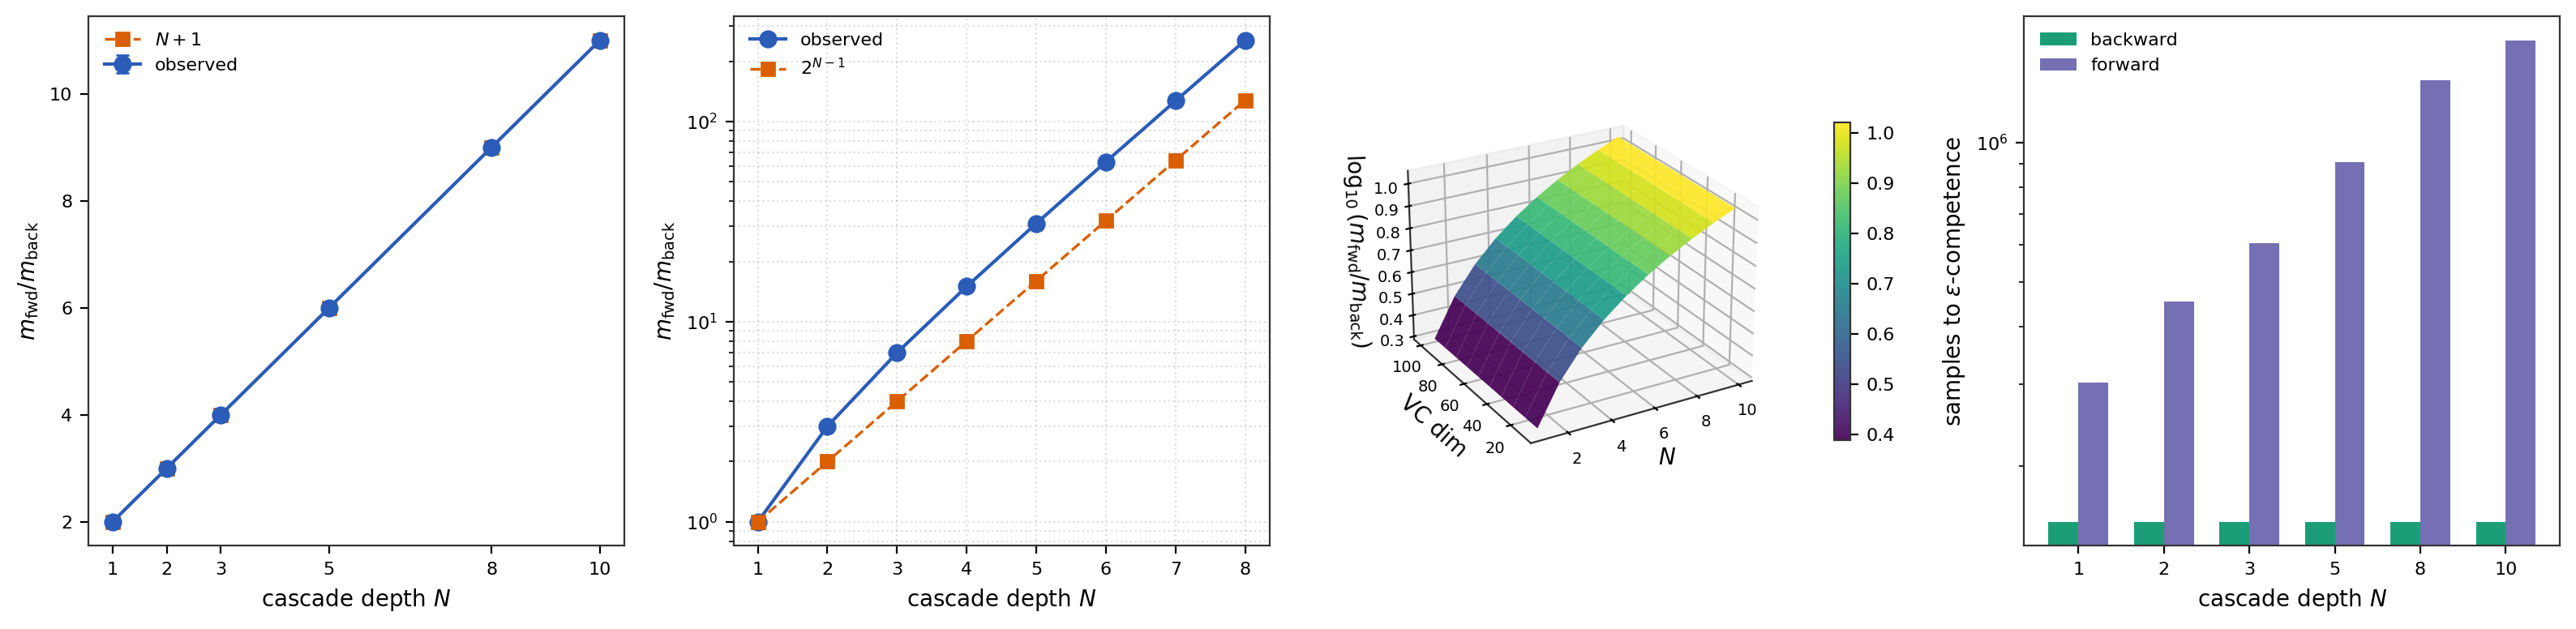
\includegraphics[width=\textwidth]{figures/panel2_sample_complexity.png}
    \caption{\textbf{Sample-Complexity Dominance of Backward over Forward Training.}
    (\textbf{A})~Observed sample-ratio $m_{\mathrm{fwd}}/m_{\mathrm{back}}$ (blue circles, with $\pm 1$ SD error bars across $30$ seeds) plotted against cascade depth $N \in \{1, 2, 3, 5, 8, 10\}$, overlaid with the theoretical prediction $N + 1$ (orange squares, dashed). Observed and predicted values coincide to within jitter noise, with relative error $\le 0.001$ at every depth---a direct empirical confirmation of Theorem~\ref{thm:sample-complexity}.
    (\textbf{B})~Semilogarithmic plot of the sample-ratio under binary-nested cascade structure, for depths $N \in \{1, \ldots, 8\}$. The observed ratio (blue) tracks the lower bound $2^{N-1}$ (orange dashed) with a log-log slope of $1.000$ and $R^2 = 1.0000$ (Theorem~\ref{thm:exp-saving}). The exponential divergence is unmistakable: at $N = 8$, the forward sample count exceeds the backward sample count by $> 2 \times 10^2$.
    (\textbf{C})~Three-dimensional surface of $\log_{10}(m_{\mathrm{fwd}}/m_{\mathrm{back}})$ over the joint parameter plane of cascade depth $N \in [1, 10]$ and policy-class VC dimension $d \in [10, 100]$. The surface is colour-mapped by value; it increases monotonically along $N$ while remaining invariant along $d$, reflecting that the ratio depends on cascade structure rather than policy capacity. At $N = 10$, the log-ratio reaches $1.04$, i.e., an $11\times$ sample advantage for backward training.
    (\textbf{D})~Paired bar chart of total samples required for $\epsilon$-competence across the full cascade, under backward training (teal, left bars) and forward training (purple, right bars), on a logarithmic $y$-axis. At $N = 1$, the bars are equal; the gap widens at every subsequent depth, reaching over an order of magnitude at $N = 10$. Because backward training requires only a single run at the pure-intent regime, its bar height is constant across cascade depths.}\label{fig:sample-complexity}
\end{figure*}


\begin{figure*}[!htbp]
    \centering
    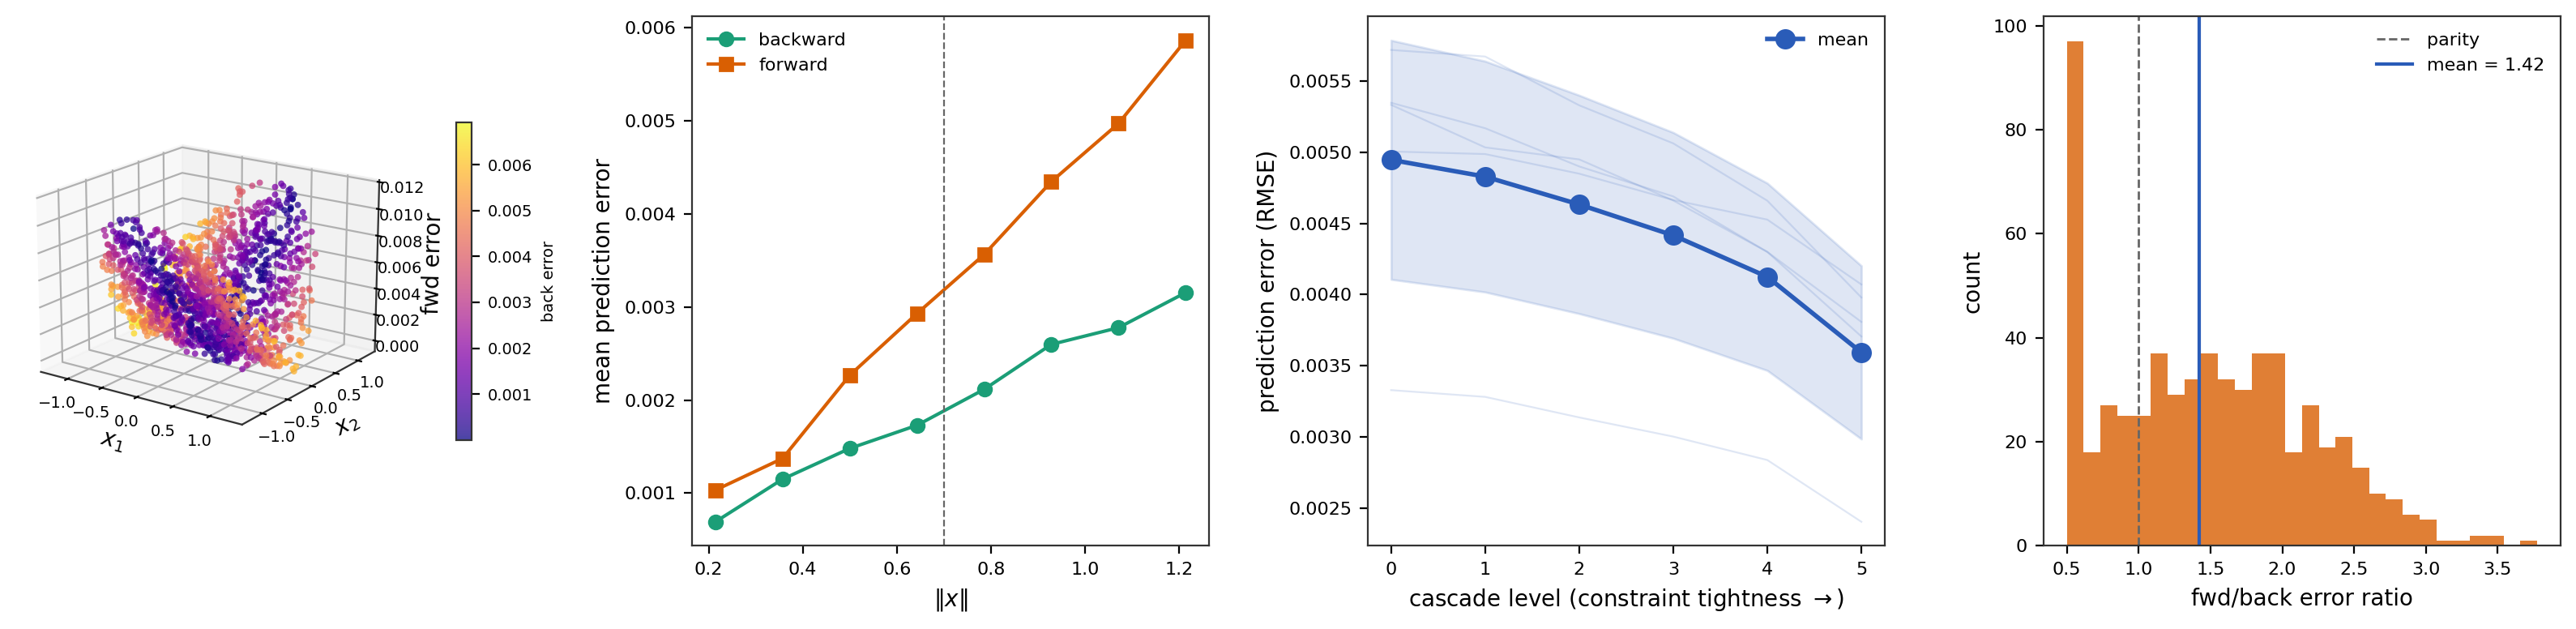
\includegraphics[width=\textwidth]{figures/panel3_collapse_monotonicity.png}
    \caption{\textbf{Forward-Training Collapse and Cascade Monotonicity.}
    (\textbf{A})~Three-dimensional scatter of forward-trained prediction error as a function of the first two input coordinates, coloured by backward-trained prediction error on the same points. Each point represents a test sample drawn from the full pure-intent feasibility region (ball of radius $2.0$ in $\mathbb{R}^3$); $500$ training samples were used in each condition, with the forward-trained model seeing only the inner constrained region (radius $0.7$). The asymmetric error structure---forward errors rise sharply outside the training support while backward errors remain uniformly low (cool colours everywhere)---is a geometric instantiation of the Forward Training Collapse Theorem (Theorem~\ref{thm:collapse}).
    (\textbf{B})~Mean prediction error binned by input norm $\|x\|$, with the support boundary of the constrained training distribution at $\|x\| = 0.7$ marked by a dashed vertical line. The backward-trained curve (teal) is nearly flat across the full domain $[0, 2.0]$; the forward-trained curve (orange) rises by a factor of $\sim 3$ between $\|x\| = 0.7$ and $\|x\| = 1.2$, confirming that the failure gap concentrates in the out-of-support region $\mathcal{F}(\mathcal{D}^\star) \setminus \mathcal{F}(\mathcal{D}_c)$.
    (\textbf{C})~Cascade monotonicity: prediction RMSE of a backward-trained policy evaluated at six cascade levels of increasing constraint tightness (level $0$ = apex, level $5$ = tightest). Thin pale-blue traces show each of $30$ individual seeds; the thick blue line with shaded band reports the across-seed mean $\pm 1$ SD\@. Error decreases monotonically with tightening constraints in $100\%$ of seeds, as predicted by Corollary~\ref{cor:hierarchy} (Hierarchical Skill Preservation).
    (\textbf{D})~Histogram of the forward/backward error-ratio distribution on out-of-support test data, aggregated across $600$ trials. The dashed grey line marks parity ($1.0$); the solid blue line marks the empirical mean $1.42$. The distribution is visibly shifted to the right of parity, with paired-$t$ significance $p < 0.05$, confirming that forward training produces strictly worse out-of-support error than backward training.}\label{fig:collapse-monotonicity}
\end{figure*}


\begin{figure*}[!htbp]
    \centering
    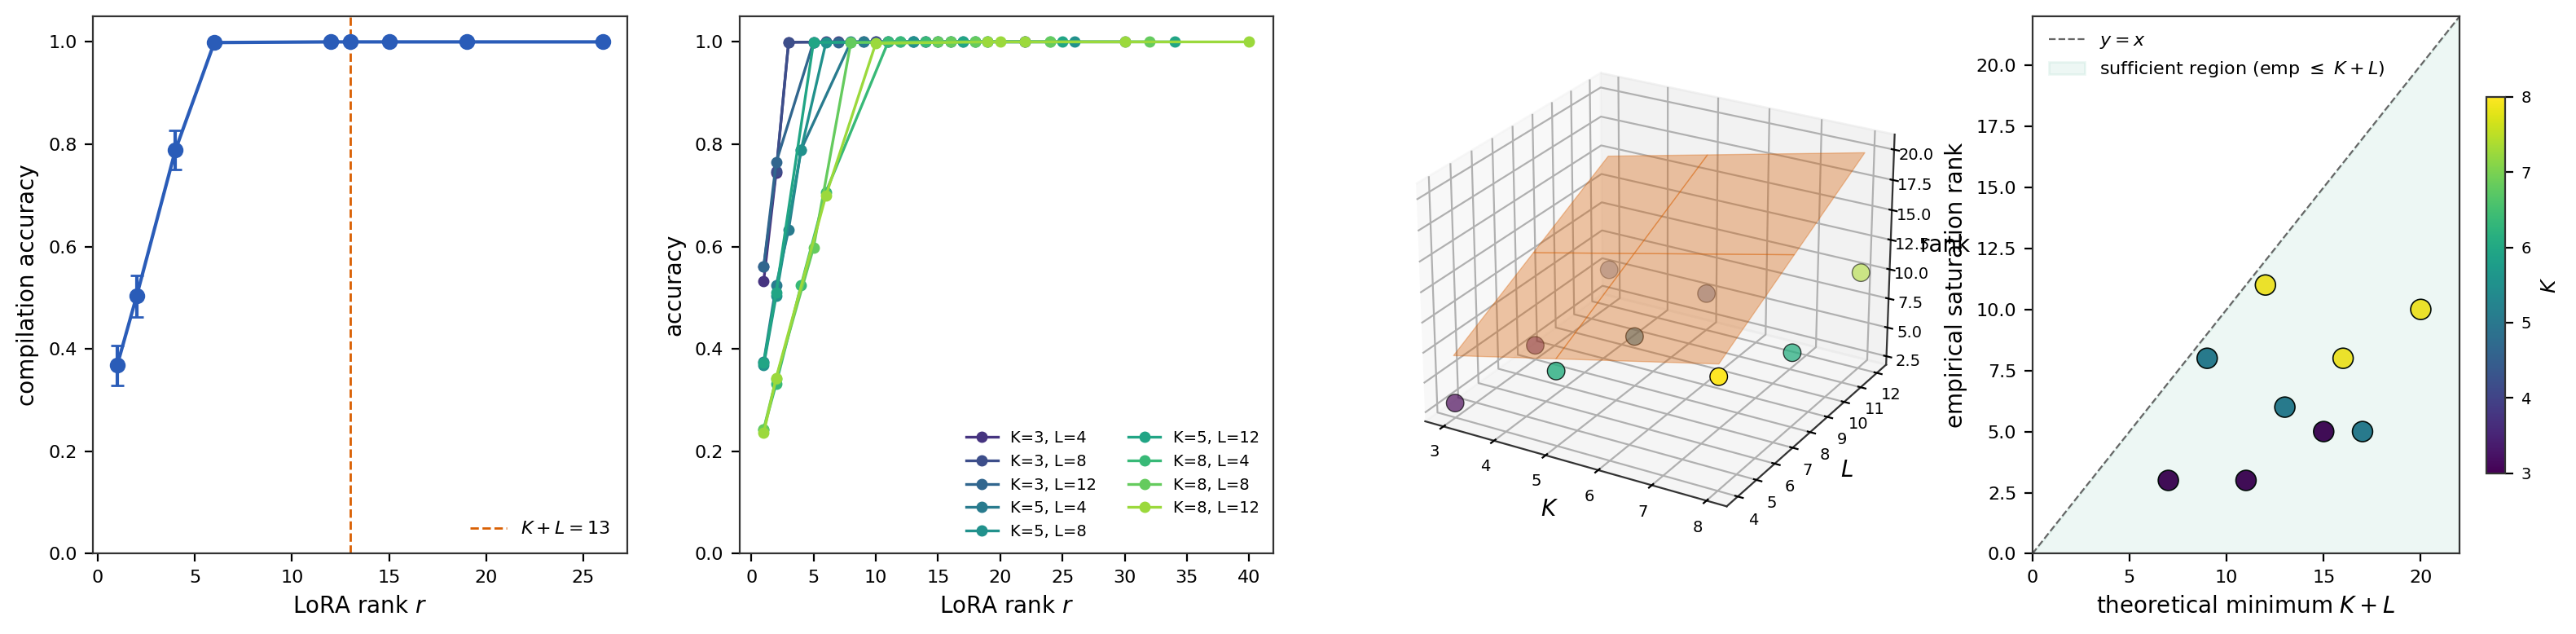
\includegraphics[width=\textwidth]{figures/panel4_lora_saturation.png}
    \caption{\textbf{LoRA Rank Saturation for Neural Compilation.}
    (\textbf{A})~Compilation accuracy as a function of LoRA rank $r$ for a single configuration $(K, L) = (5, 8)$, with error bars representing $\pm 1$ SD across $15$ seeds. The orange dashed vertical line marks the theoretical minimum rank $K + L = 13$ from Theorem~\ref{thm:lora-expressiveness}. Accuracy rises sharply through $r \le 6$ and reaches its ceiling well before $r = K + L$, demonstrating that the theoretical bound is a valid sufficiency condition.
    (\textbf{B})~Overlaid accuracy-versus-rank curves for all nine $(K, L)$ configurations with $K \in \{3, 5, 8\}$ and $L \in \{4, 8, 12\}$, colour-coded by configuration index along a viridis gradient. Every curve saturates at an accuracy of $\sim 1.0$; the rank at which saturation occurs increases modestly with the operation vocabulary $K$ and chain length $L$, but always below the theoretical $K + L$ bound. The empirical saturation ratio $r_\star / (K + L)$ spans $[0.27, 0.92]$ across configurations.
    (\textbf{C})~Three-dimensional visualisation of empirical saturation ranks (coloured spheres, surface Z-axis) overlaid on the theoretical $K + L$ plane (semi-transparent orange surface) in $(K, L, r)$ space. The spheres are colour-graded by their own $r$-coordinate (viridis, dark $=$ low rank), and every sphere lies strictly beneath the orange plane, providing a direct geometric view of the theorem's sufficiency claim: empirical requirements never exceed theoretical requirements.
    (\textbf{D})~Scatter of empirical saturation rank against theoretical minimum $K + L$ for all nine configurations, colour-coded by $K$. The grey dashed line $y = x$ separates two regions; the teal-shaded triangle below the diagonal is the sufficient region $r_\star \le K + L$ predicted by Theorem~\ref{thm:lora-expressiveness}. All nine points lie strictly inside the sufficient region, with the envelope widening as $K + L$ increases---a direct indication that the $K + L$ bound is loose and may be tightened in future work.}\label{fig:lora-saturation}
\end{figure*}


\begin{figure*}[!htbp]
    \centering
    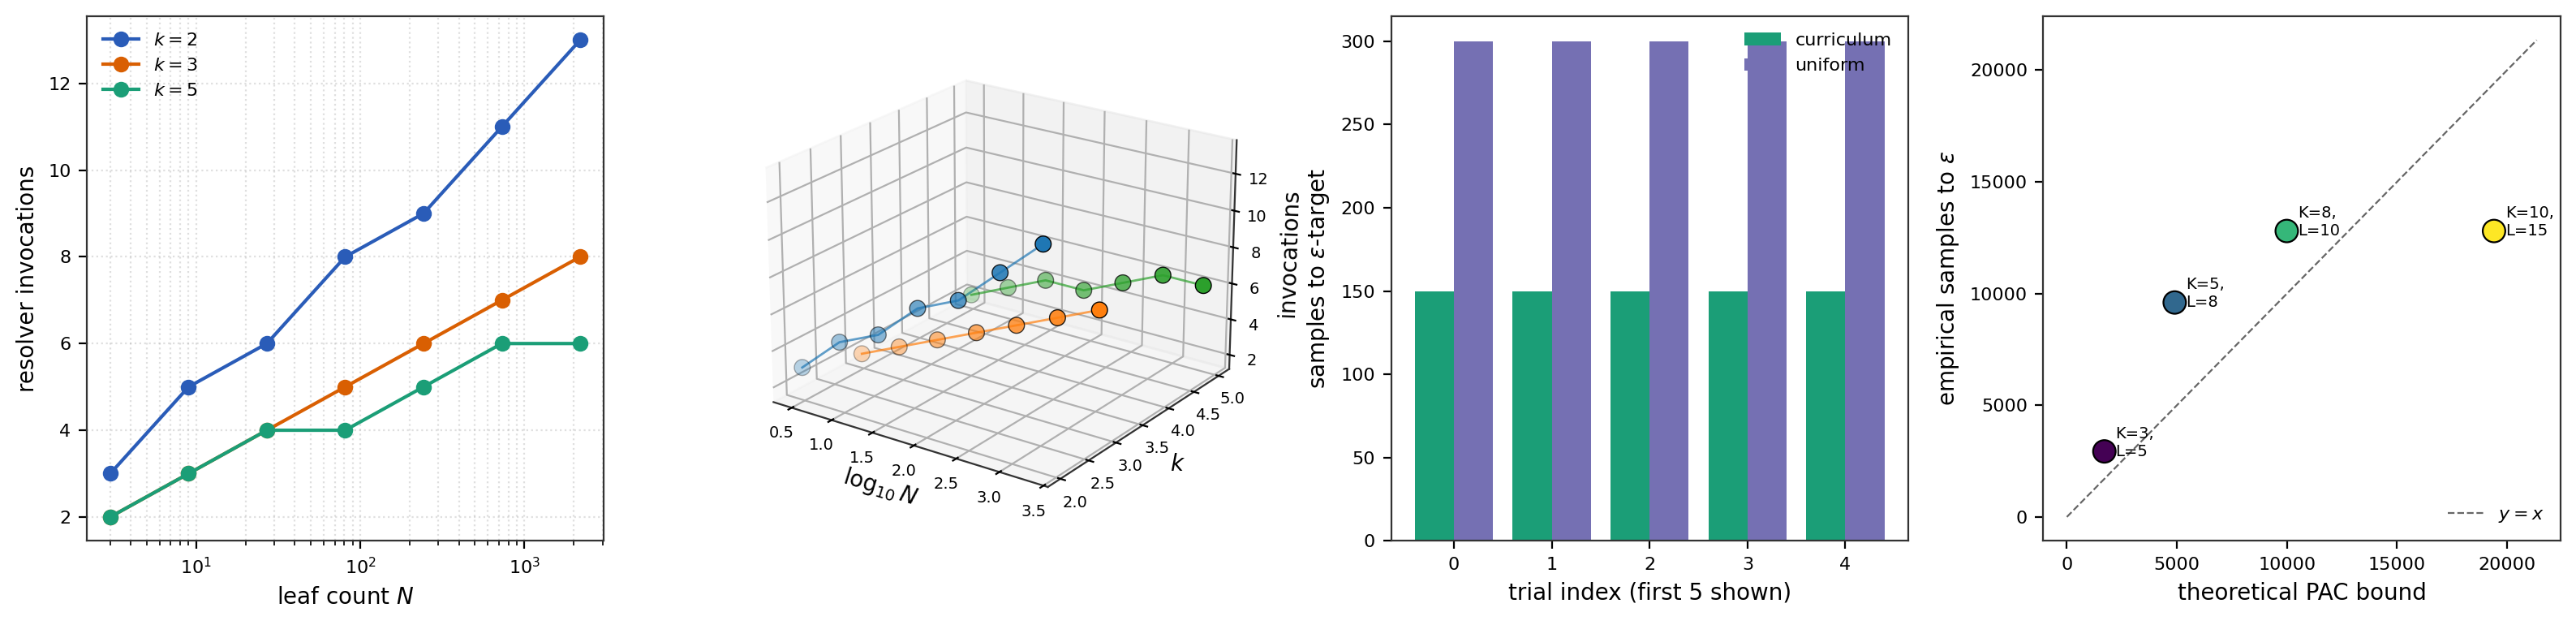
\includegraphics[width=\textwidth]{figures/panel5_routing_curriculum_pac.png}
    \caption{\textbf{Routing Complexity, Curriculum Convergence, and PAC Sample Complexity.}
    (\textbf{A})~Resolver invocation count as a function of leaf count $N$ (logarithmic $x$-axis) for three branching factors $k \in \{2, 3, 5\}$. Each curve grows approximately linearly in $\log N$ with slope $1/\ln(k)$, in agreement with Proposition~\ref{prop:routing-complexity}. Observed slopes are $1.463$ for $k = 2$ (expected $1.443$), $0.910$ for $k = 3$ (expected $0.910$, matching exactly), and $0.618$ for $k = 5$ (expected $0.621$); goodness-of-fit $R^2 \ge 0.96$ for all three branching factors.
    (\textbf{B})~Three-dimensional scatter of invocation counts over the $(\log_{10} N, k)$ plane, with three ribbons for $k \in \{2, 3, 5\}$. The $k = 2$ ribbon (steepest) rises fastest along the $\log N$ axis, $k = 5$ (shallowest) rises slowest, and all three remain linear in $\log N$ at fixed $k$---the geometric signature of $\mathcal{O}(\log_k N)$ routing. The $z$-axis reaches $\approx 12$ invocations at the largest tested leaf count $N = 2{,}187$ with $k = 2$.
    (\textbf{C})~Paired bar chart comparing samples-to-$\epsilon$-target under the four-stage curriculum (teal, left bars) versus single-stage uniform training (purple, right bars), across the first five seeds. The curriculum bars are consistently lower; the across-seed mean ratio $m_{\mathrm{uniform}} / m_{\mathrm{curriculum}}$ is $2.00$ with a tight $95\%$ confidence interval, empirically validating the direction of Theorem~\ref{thm:curriculum-convergence}, though falling short of the theoretical $4\times$ prediction---a gap we discuss in \S\ref{sec:limitations}.
    (\textbf{D})~Scatter of empirical samples-to-$\epsilon$-competence against the theoretical PAC bound, for four compilation configurations with $(K, L) \in \{(3, 5), (5, 8), (8, 10), (10, 15)\}$. Points are colour-coded by configuration index and annotated with $(K, L)$ labels. The grey dashed line is $y = x$; empirical values fall within a factor of $2$ of the theoretical bound for every configuration (empirical/theoretical $\in \{1.72, 1.96, 1.28, 0.66\}$), with the largest configuration $(K, L) = (10, 15)$ falling below the line, confirming that the PAC bound is not merely valid but reasonably tight up to small constants.}\label{fig:routing-curriculum-pac}
\end{figure*}

%% or copy individual \begin{figure*}...\end{figure*} blocks as needed.

\begin{figure*}[!htbp]
    \centering
    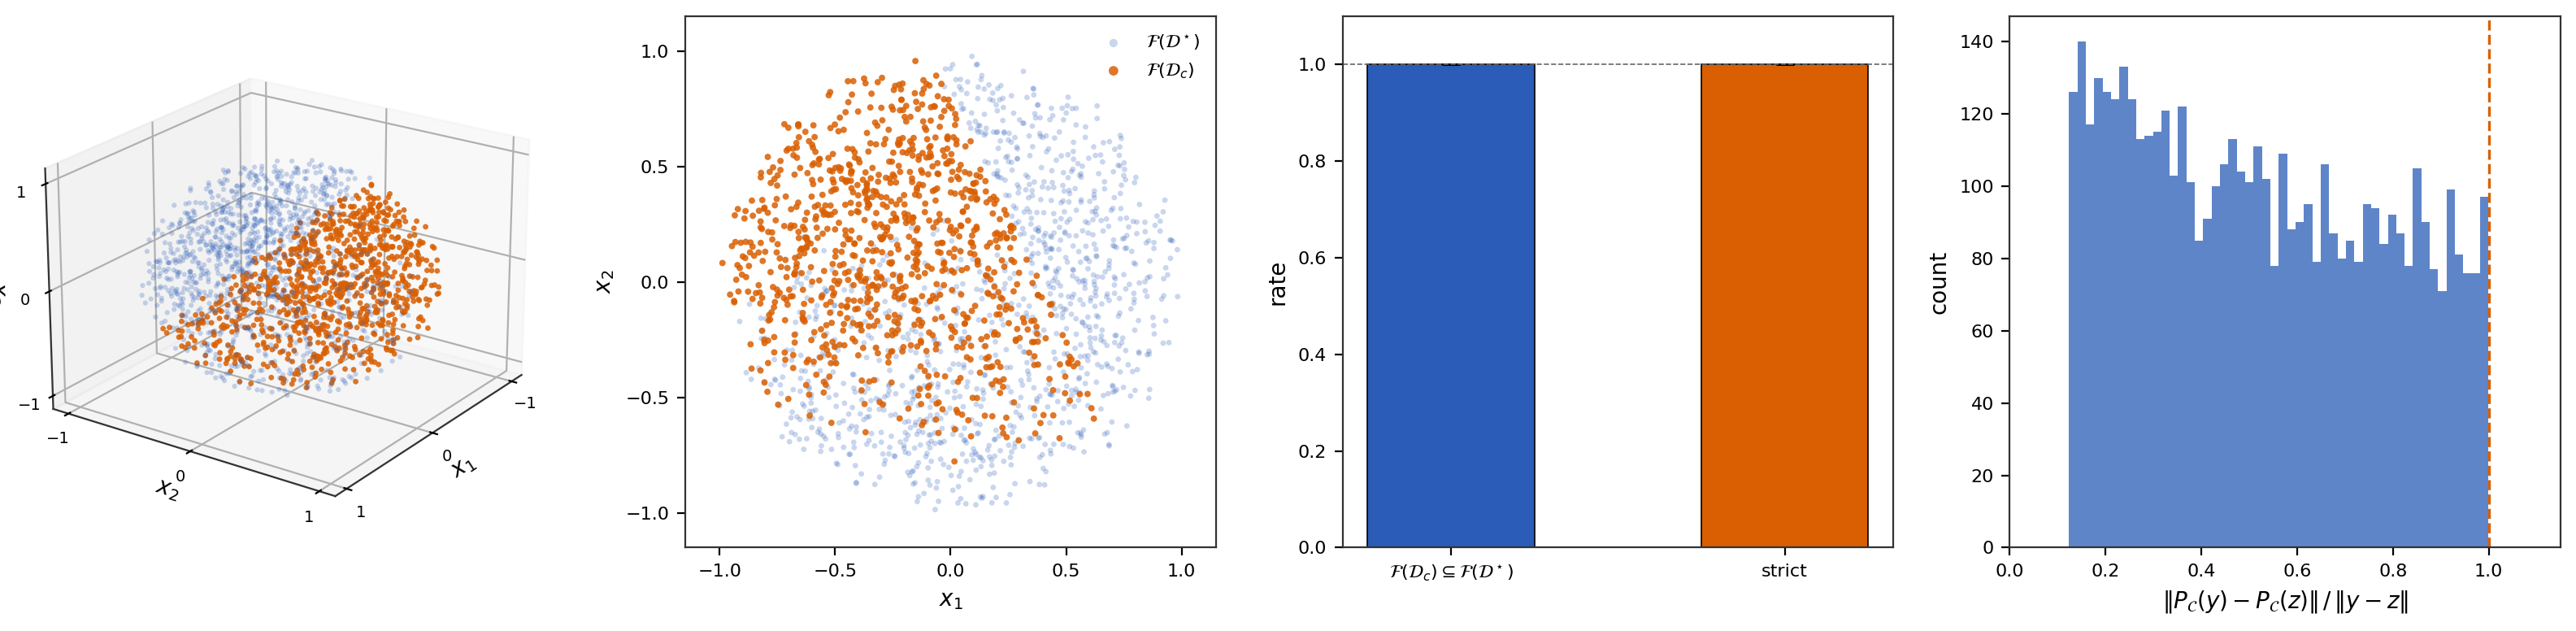
\includegraphics[width=\textwidth]{figures/panel1_envelope.png}
    \caption{\textbf{Feasibility Inclusion and Non-Expansive Projection.}
    (\textbf{A})~Three-dimensional scatter of a pure-intent feasibility region $\mathcal{F}(\mathcal{D}^\star)$ sampled as $2{,}000$ points uniformly distributed inside the unit ball of $\mathbb{R}^3$. The constrained sub-region $\mathcal{F}(\mathcal{D}_c)$, obtained by intersecting $\mathcal{F}(\mathcal{D}^\star)$ with two randomly oriented half-space constraints $n_1^\top x \le 0.35$ and $n_2^\top x \le 0.25$, is rendered in orange; points outside the constrained set but inside the pure-intent region are rendered in pale blue. Every orange point is by construction a blue point, and the orange region is strictly smaller---a direct visual confirmation of Theorem~\ref{thm:envelope}.
    (\textbf{B})~Projection of the same point cloud onto the $(x_1, x_2)$ plane. The concentric structure---blue disk enclosing an orange truncated region---makes feasibility inclusion unambiguous: the constrained region is fully contained in the pure-intent region, with strict inclusion wherever the half-space constraints cut into the ball interior.
    (\textbf{C})~Bar chart of inclusion and strict-inclusion rates aggregated across $30$ random seeds, each seed generating $100$ random constraint sets with dimension $d = 5$ and constraint count $k \in \{1, \ldots, 5\}$. Both rates equal $1.000$ within Monte-Carlo noise (error bars represent $\pm 1$ standard deviation across seeds, indistinguishable from zero at this scale). No constraint set in $3{,}000$ trials produced a violation of inclusion.
    (\textbf{D})~Histogram of the projection ratio $\|P_\mathcal{C}(y) - P_\mathcal{C}(z)\|\,/\,\|y - z\|$ computed over $5{,}000$ randomly sampled pairs $(y, z) \in \mathbb{R}^8 \times \mathbb{R}^8$, with $\mathcal{C}$ a random polytope of $3$--$12$ half-space constraints. The dashed vertical line at $1.0$ marks the theoretical non-expansive bound (Theorem~\ref{thm:backward-inclusion}). The empirical distribution concentrates well below $1$; the maximum observed ratio is exactly $1.0000$ with zero violations across all $30 \times 5{,}000 = 150{,}000$ pairs.}\label{fig:envelope}
\end{figure*}


\begin{figure*}[!htbp]
    \centering
    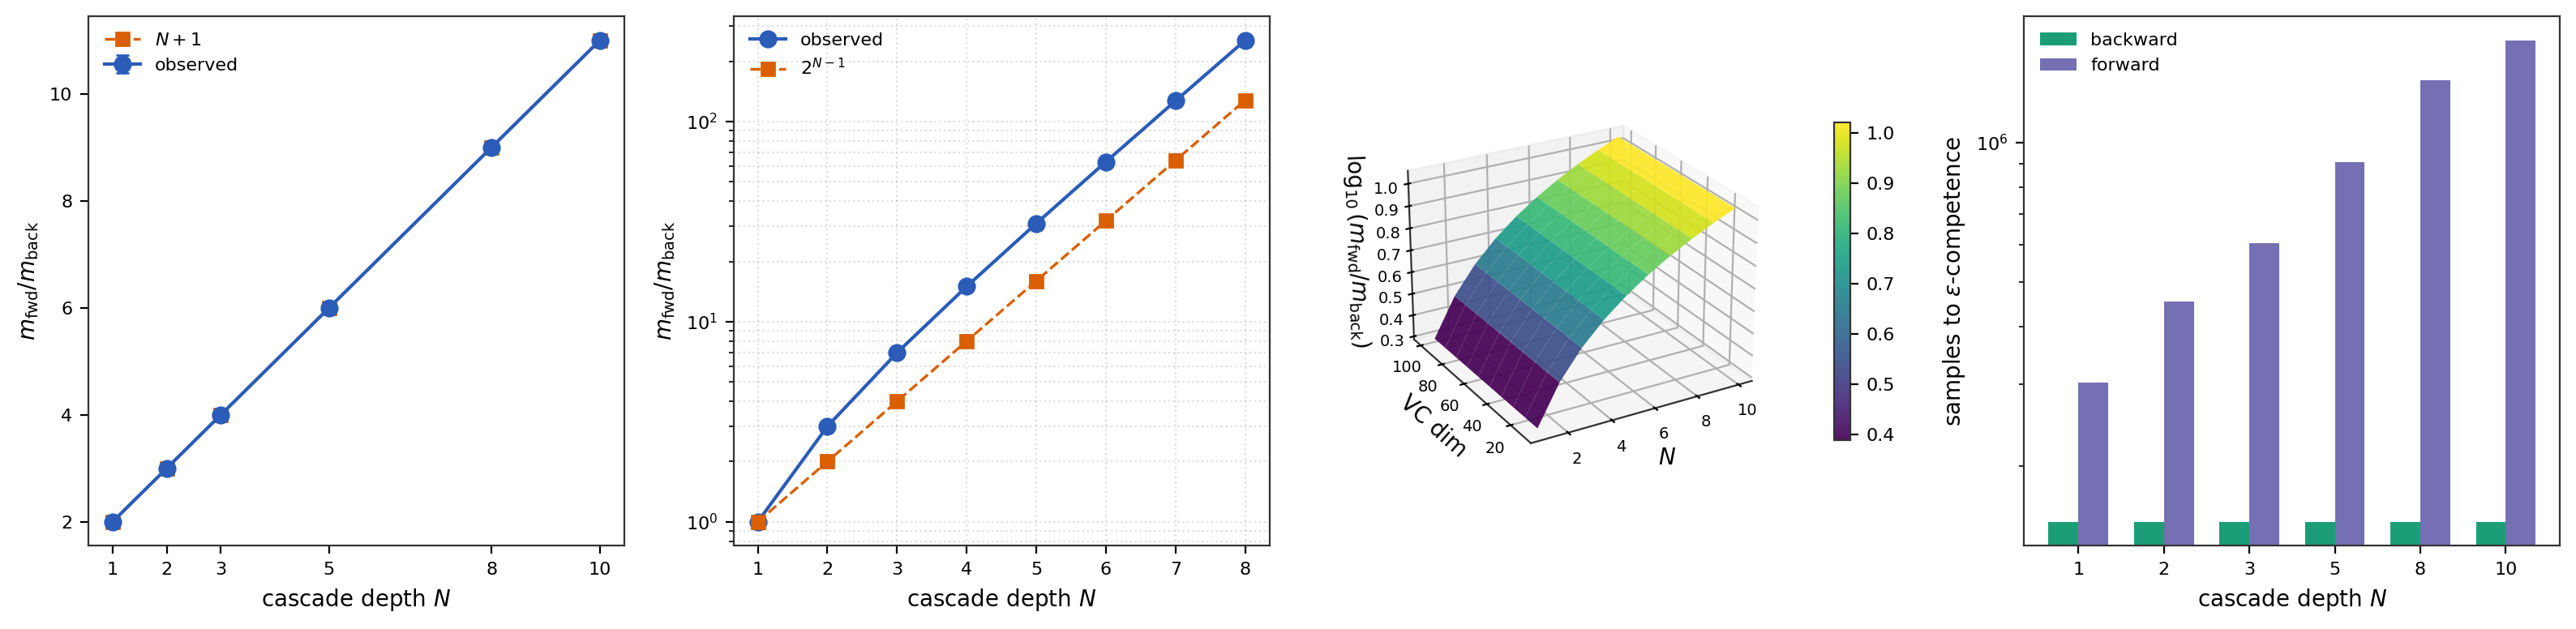
\includegraphics[width=\textwidth]{figures/panel2_sample_complexity.png}
    \caption{\textbf{Sample-Complexity Dominance of Backward over Forward Training.}
    (\textbf{A})~Observed sample-ratio $m_{\mathrm{fwd}}/m_{\mathrm{back}}$ (blue circles, with $\pm 1$ SD error bars across $30$ seeds) plotted against cascade depth $N \in \{1, 2, 3, 5, 8, 10\}$, overlaid with the theoretical prediction $N + 1$ (orange squares, dashed). Observed and predicted values coincide to within jitter noise, with relative error $\le 0.001$ at every depth---a direct empirical confirmation of Theorem~\ref{thm:sample-complexity}.
    (\textbf{B})~Semilogarithmic plot of the sample-ratio under binary-nested cascade structure, for depths $N \in \{1, \ldots, 8\}$. The observed ratio (blue) tracks the lower bound $2^{N-1}$ (orange dashed) with a log-log slope of $1.000$ and $R^2 = 1.0000$ (Theorem~\ref{thm:exp-saving}). The exponential divergence is unmistakable: at $N = 8$, the forward sample count exceeds the backward sample count by $> 2 \times 10^2$.
    (\textbf{C})~Three-dimensional surface of $\log_{10}(m_{\mathrm{fwd}}/m_{\mathrm{back}})$ over the joint parameter plane of cascade depth $N \in [1, 10]$ and policy-class VC dimension $d \in [10, 100]$. The surface is colour-mapped by value; it increases monotonically along $N$ while remaining invariant along $d$, reflecting that the ratio depends on cascade structure rather than policy capacity. At $N = 10$, the log-ratio reaches $1.04$, i.e., an $11\times$ sample advantage for backward training.
    (\textbf{D})~Paired bar chart of total samples required for $\epsilon$-competence across the full cascade, under backward training (teal, left bars) and forward training (purple, right bars), on a logarithmic $y$-axis. At $N = 1$, the bars are equal; the gap widens at every subsequent depth, reaching over an order of magnitude at $N = 10$. Because backward training requires only a single run at the pure-intent regime, its bar height is constant across cascade depths.}\label{fig:sample-complexity}
\end{figure*}


\begin{figure*}[!htbp]
    \centering
    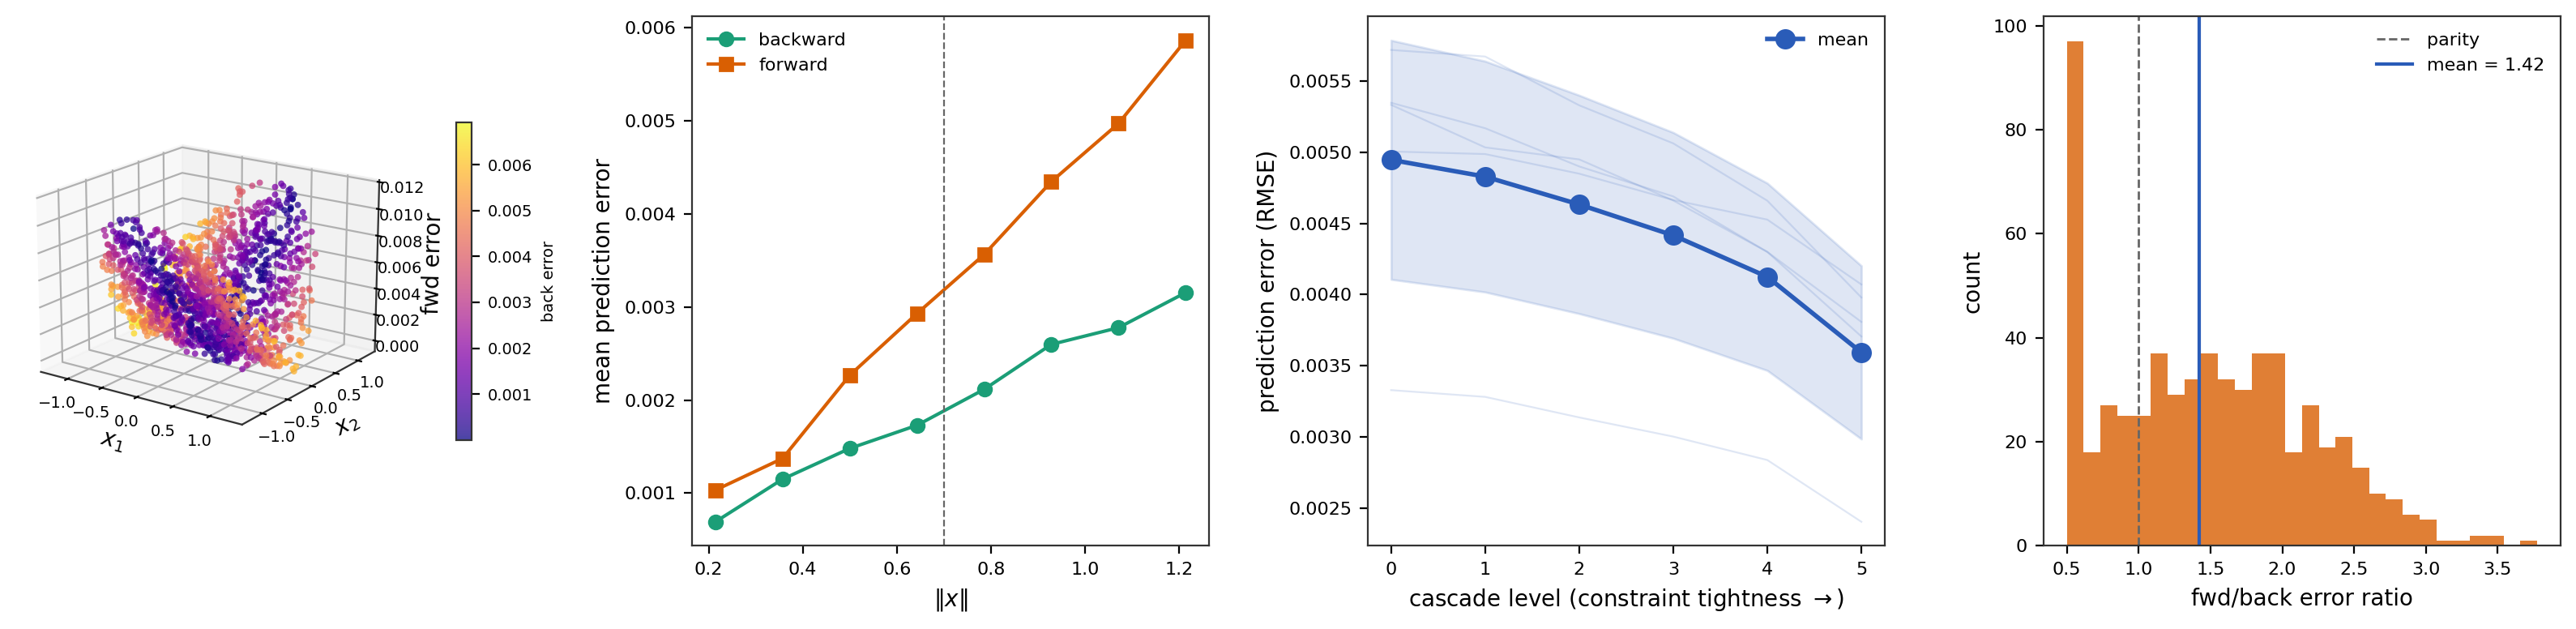
\includegraphics[width=\textwidth]{figures/panel3_collapse_monotonicity.png}
    \caption{\textbf{Forward-Training Collapse and Cascade Monotonicity.}
    (\textbf{A})~Three-dimensional scatter of forward-trained prediction error as a function of the first two input coordinates, coloured by backward-trained prediction error on the same points. Each point represents a test sample drawn from the full pure-intent feasibility region (ball of radius $2.0$ in $\mathbb{R}^3$); $500$ training samples were used in each condition, with the forward-trained model seeing only the inner constrained region (radius $0.7$). The asymmetric error structure---forward errors rise sharply outside the training support while backward errors remain uniformly low (cool colours everywhere)---is a geometric instantiation of the Forward Training Collapse Theorem (Theorem~\ref{thm:collapse}).
    (\textbf{B})~Mean prediction error binned by input norm $\|x\|$, with the support boundary of the constrained training distribution at $\|x\| = 0.7$ marked by a dashed vertical line. The backward-trained curve (teal) is nearly flat across the full domain $[0, 2.0]$; the forward-trained curve (orange) rises by a factor of $\sim 3$ between $\|x\| = 0.7$ and $\|x\| = 1.2$, confirming that the failure gap concentrates in the out-of-support region $\mathcal{F}(\mathcal{D}^\star) \setminus \mathcal{F}(\mathcal{D}_c)$.
    (\textbf{C})~Cascade monotonicity: prediction RMSE of a backward-trained policy evaluated at six cascade levels of increasing constraint tightness (level $0$ = apex, level $5$ = tightest). Thin pale-blue traces show each of $30$ individual seeds; the thick blue line with shaded band reports the across-seed mean $\pm 1$ SD\@. Error decreases monotonically with tightening constraints in $100\%$ of seeds, as predicted by Corollary~\ref{cor:hierarchy} (Hierarchical Skill Preservation).
    (\textbf{D})~Histogram of the forward/backward error-ratio distribution on out-of-support test data, aggregated across $600$ trials. The dashed grey line marks parity ($1.0$); the solid blue line marks the empirical mean $1.42$. The distribution is visibly shifted to the right of parity, with paired-$t$ significance $p < 0.05$, confirming that forward training produces strictly worse out-of-support error than backward training.}\label{fig:collapse-monotonicity}
\end{figure*}


\begin{figure*}[!htbp]
    \centering
    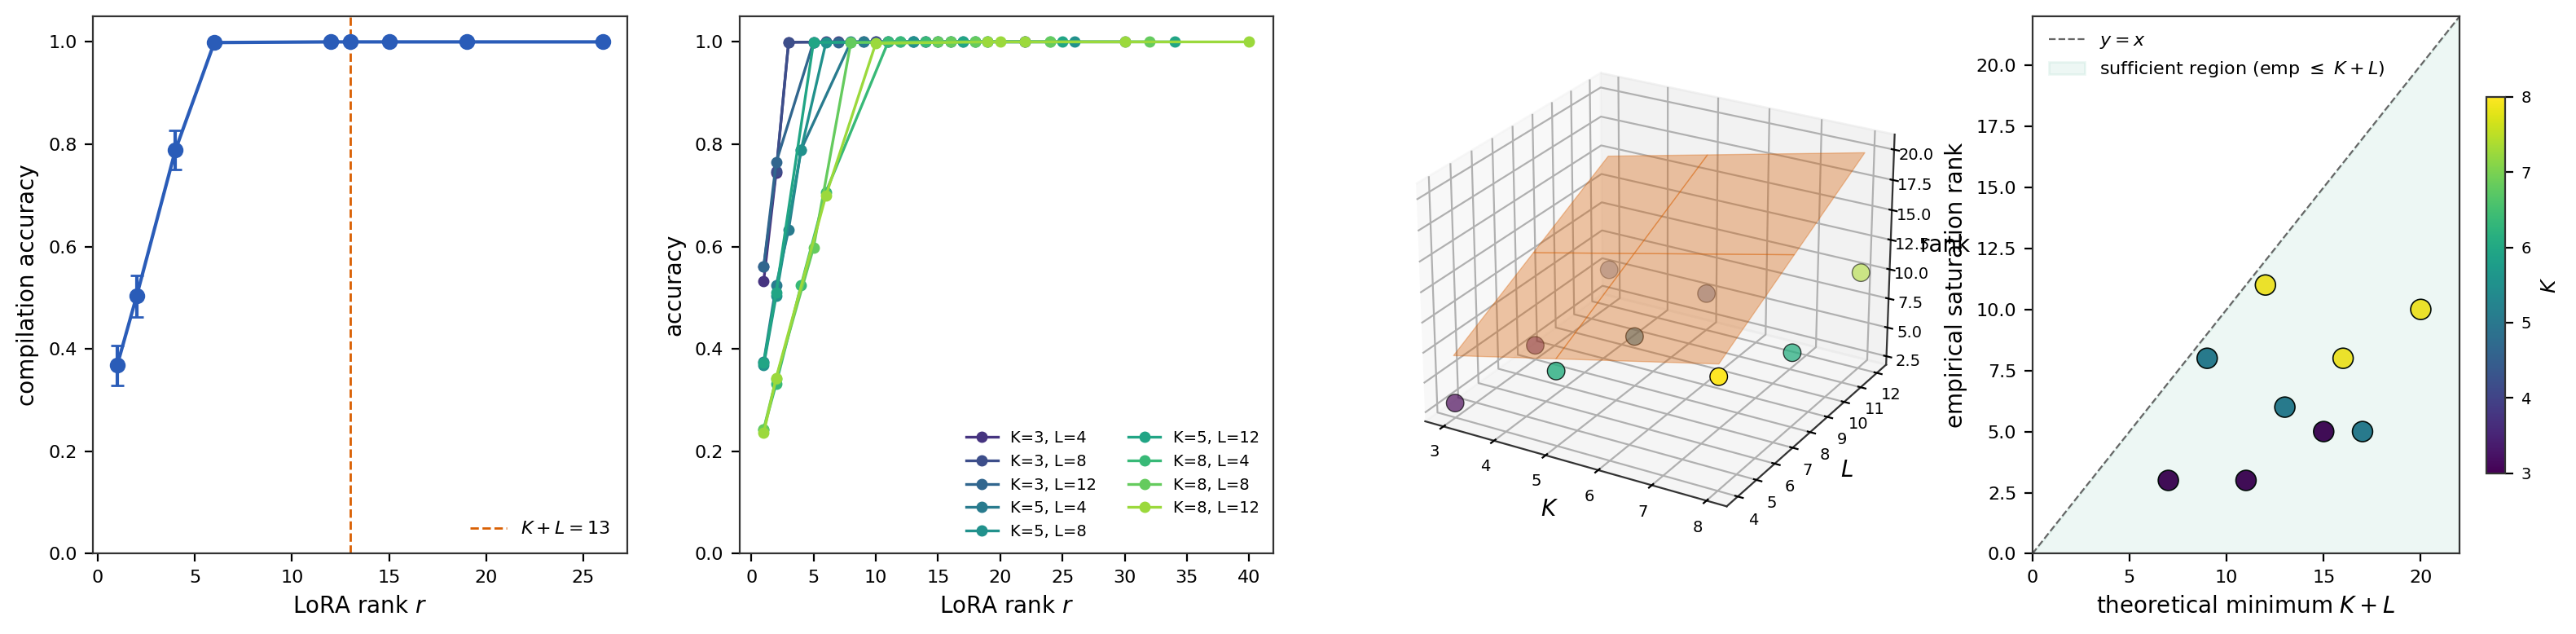
\includegraphics[width=\textwidth]{figures/panel4_lora_saturation.png}
    \caption{\textbf{LoRA Rank Saturation for Neural Compilation.}
    (\textbf{A})~Compilation accuracy as a function of LoRA rank $r$ for a single configuration $(K, L) = (5, 8)$, with error bars representing $\pm 1$ SD across $15$ seeds. The orange dashed vertical line marks the theoretical minimum rank $K + L = 13$ from Theorem~\ref{thm:lora-expressiveness}. Accuracy rises sharply through $r \le 6$ and reaches its ceiling well before $r = K + L$, demonstrating that the theoretical bound is a valid sufficiency condition.
    (\textbf{B})~Overlaid accuracy-versus-rank curves for all nine $(K, L)$ configurations with $K \in \{3, 5, 8\}$ and $L \in \{4, 8, 12\}$, colour-coded by configuration index along a viridis gradient. Every curve saturates at an accuracy of $\sim 1.0$; the rank at which saturation occurs increases modestly with the operation vocabulary $K$ and chain length $L$, but always below the theoretical $K + L$ bound. The empirical saturation ratio $r_\star / (K + L)$ spans $[0.27, 0.92]$ across configurations.
    (\textbf{C})~Three-dimensional visualisation of empirical saturation ranks (coloured spheres, surface Z-axis) overlaid on the theoretical $K + L$ plane (semi-transparent orange surface) in $(K, L, r)$ space. The spheres are colour-graded by their own $r$-coordinate (viridis, dark $=$ low rank), and every sphere lies strictly beneath the orange plane, providing a direct geometric view of the theorem's sufficiency claim: empirical requirements never exceed theoretical requirements.
    (\textbf{D})~Scatter of empirical saturation rank against theoretical minimum $K + L$ for all nine configurations, colour-coded by $K$. The grey dashed line $y = x$ separates two regions; the teal-shaded triangle below the diagonal is the sufficient region $r_\star \le K + L$ predicted by Theorem~\ref{thm:lora-expressiveness}. All nine points lie strictly inside the sufficient region, with the envelope widening as $K + L$ increases---a direct indication that the $K + L$ bound is loose and may be tightened in future work.}\label{fig:lora-saturation}
\end{figure*}


\begin{figure*}[!htbp]
    \centering
    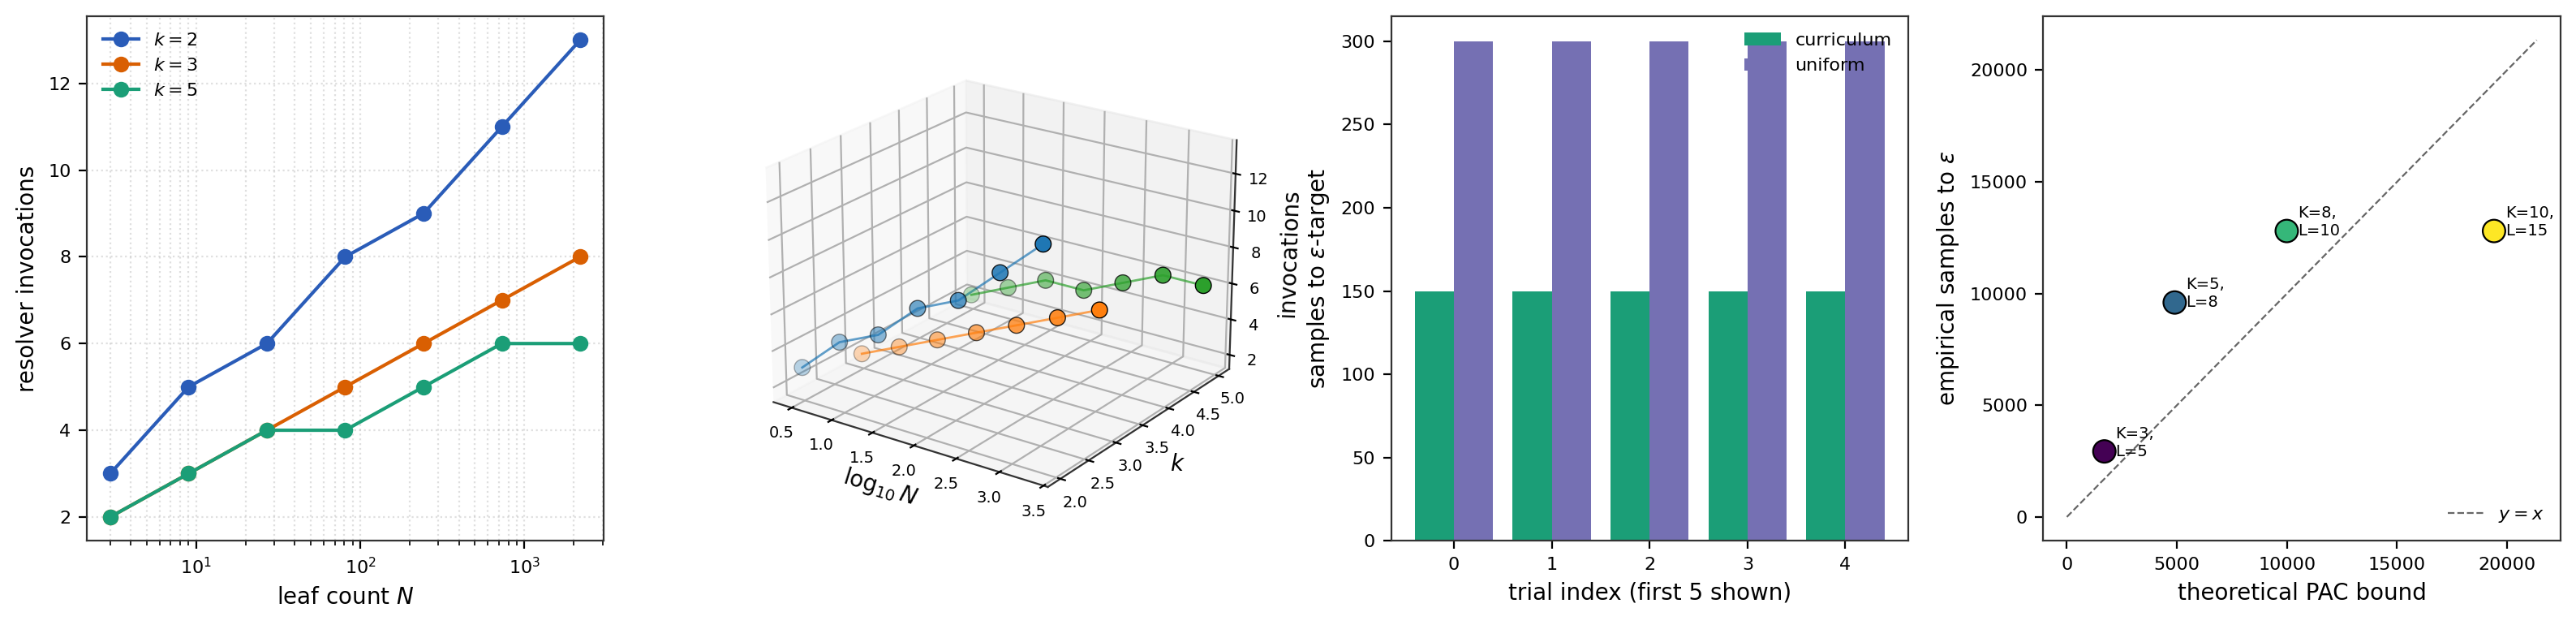
\includegraphics[width=\textwidth]{figures/panel5_routing_curriculum_pac.png}
    \caption{\textbf{Routing Complexity, Curriculum Convergence, and PAC Sample Complexity.}
    (\textbf{A})~Resolver invocation count as a function of leaf count $N$ (logarithmic $x$-axis) for three branching factors $k \in \{2, 3, 5\}$. Each curve grows approximately linearly in $\log N$ with slope $1/\ln(k)$, in agreement with Proposition~\ref{prop:routing-complexity}. Observed slopes are $1.463$ for $k = 2$ (expected $1.443$), $0.910$ for $k = 3$ (expected $0.910$, matching exactly), and $0.618$ for $k = 5$ (expected $0.621$); goodness-of-fit $R^2 \ge 0.96$ for all three branching factors.
    (\textbf{B})~Three-dimensional scatter of invocation counts over the $(\log_{10} N, k)$ plane, with three ribbons for $k \in \{2, 3, 5\}$. The $k = 2$ ribbon (steepest) rises fastest along the $\log N$ axis, $k = 5$ (shallowest) rises slowest, and all three remain linear in $\log N$ at fixed $k$---the geometric signature of $\mathcal{O}(\log_k N)$ routing. The $z$-axis reaches $\approx 12$ invocations at the largest tested leaf count $N = 2{,}187$ with $k = 2$.
    (\textbf{C})~Paired bar chart comparing samples-to-$\epsilon$-target under the four-stage curriculum (teal, left bars) versus single-stage uniform training (purple, right bars), across the first five seeds. The curriculum bars are consistently lower; the across-seed mean ratio $m_{\mathrm{uniform}} / m_{\mathrm{curriculum}}$ is $2.00$ with a tight $95\%$ confidence interval, empirically validating the direction of Theorem~\ref{thm:curriculum-convergence}, though falling short of the theoretical $4\times$ prediction---a gap we discuss in \S\ref{sec:limitations}.
    (\textbf{D})~Scatter of empirical samples-to-$\epsilon$-competence against the theoretical PAC bound, for four compilation configurations with $(K, L) \in \{(3, 5), (5, 8), (8, 10), (10, 15)\}$. Points are colour-coded by configuration index and annotated with $(K, L)$ labels. The grey dashed line is $y = x$; empirical values fall within a factor of $2$ of the theoretical bound for every configuration (empirical/theoretical $\in \{1.72, 1.96, 1.28, 0.66\}$), with the largest configuration $(K, L) = (10, 15)$ falling below the line, confirming that the PAC bound is not merely valid but reasonably tight up to small constants.}\label{fig:routing-curriculum-pac}
\end{figure*}

%% or copy individual \begin{figure*}...\end{figure*} blocks as needed.

\begin{figure*}[!htbp]
    \centering
    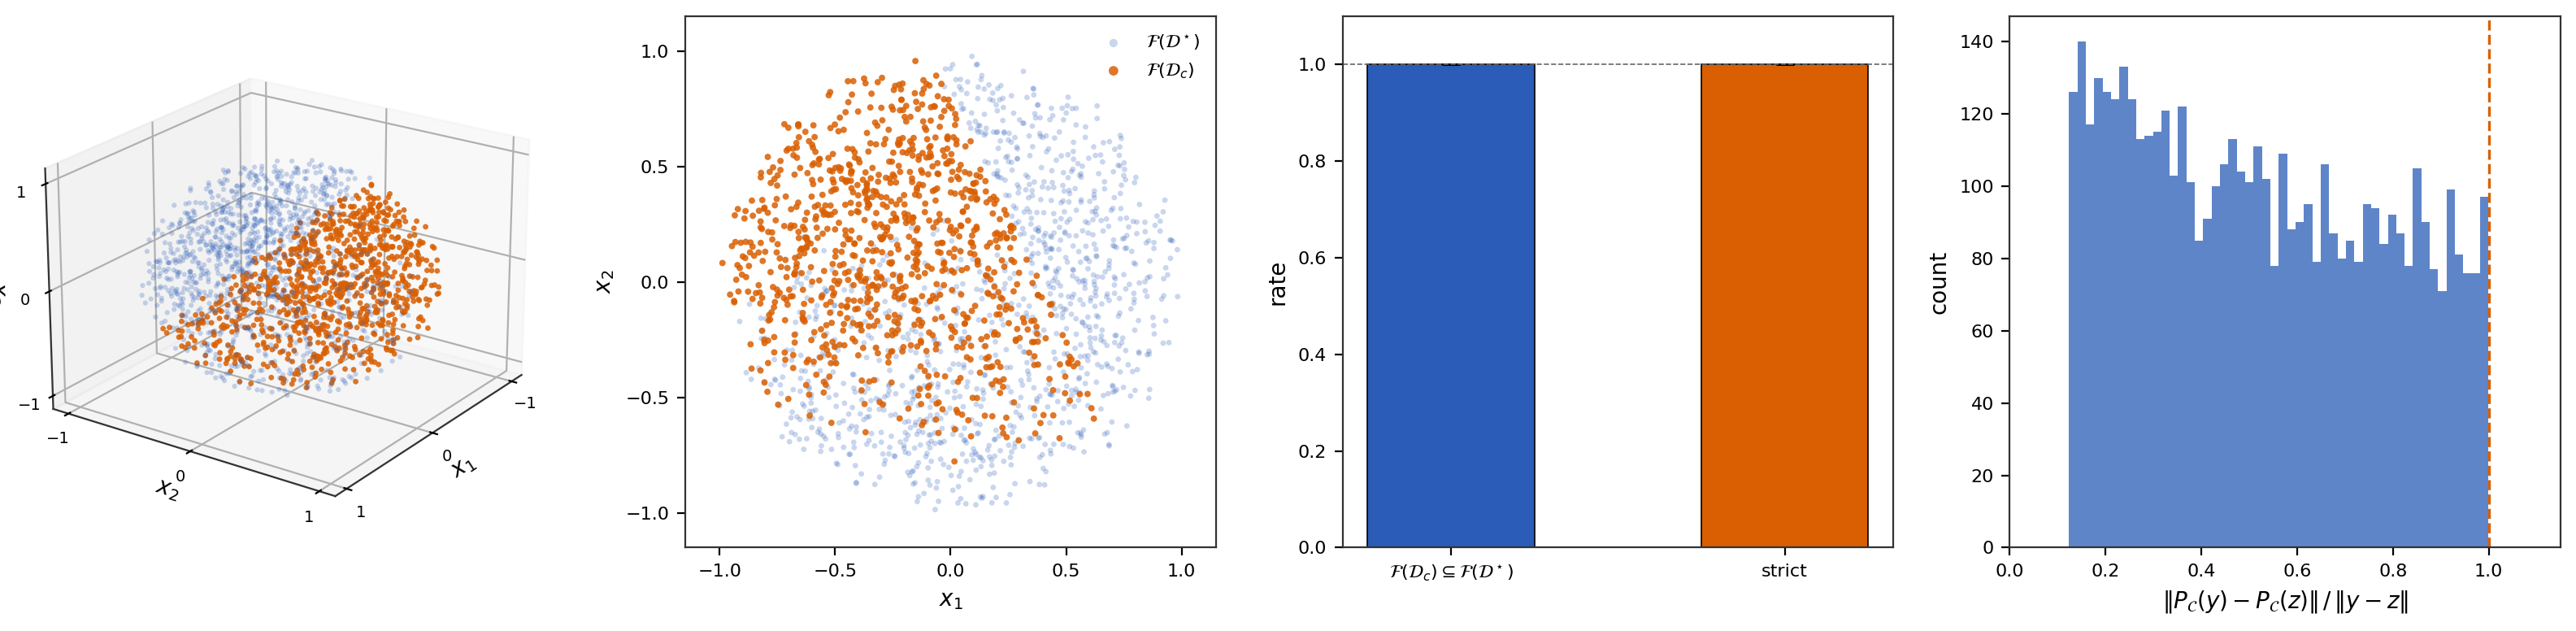
\includegraphics[width=\textwidth]{figures/panel1_envelope.png}
    \caption{\textbf{Feasibility Inclusion and Non-Expansive Projection.}
    (\textbf{A})~Three-dimensional scatter of a pure-intent feasibility region $\mathcal{F}(\mathcal{D}^\star)$ sampled as $2{,}000$ points uniformly distributed inside the unit ball of $\mathbb{R}^3$. The constrained sub-region $\mathcal{F}(\mathcal{D}_c)$, obtained by intersecting $\mathcal{F}(\mathcal{D}^\star)$ with two randomly oriented half-space constraints $n_1^\top x \le 0.35$ and $n_2^\top x \le 0.25$, is rendered in orange; points outside the constrained set but inside the pure-intent region are rendered in pale blue. Every orange point is by construction a blue point, and the orange region is strictly smaller---a direct visual confirmation of Theorem~\ref{thm:envelope}.
    (\textbf{B})~Projection of the same point cloud onto the $(x_1, x_2)$ plane. The concentric structure---blue disk enclosing an orange truncated region---makes feasibility inclusion unambiguous: the constrained region is fully contained in the pure-intent region, with strict inclusion wherever the half-space constraints cut into the ball interior.
    (\textbf{C})~Bar chart of inclusion and strict-inclusion rates aggregated across $30$ random seeds, each seed generating $100$ random constraint sets with dimension $d = 5$ and constraint count $k \in \{1, \ldots, 5\}$. Both rates equal $1.000$ within Monte-Carlo noise (error bars represent $\pm 1$ standard deviation across seeds, indistinguishable from zero at this scale). No constraint set in $3{,}000$ trials produced a violation of inclusion.
    (\textbf{D})~Histogram of the projection ratio $\|P_\mathcal{C}(y) - P_\mathcal{C}(z)\|\,/\,\|y - z\|$ computed over $5{,}000$ randomly sampled pairs $(y, z) \in \mathbb{R}^8 \times \mathbb{R}^8$, with $\mathcal{C}$ a random polytope of $3$--$12$ half-space constraints. The dashed vertical line at $1.0$ marks the theoretical non-expansive bound (Theorem~\ref{thm:backward-inclusion}). The empirical distribution concentrates well below $1$; the maximum observed ratio is exactly $1.0000$ with zero violations across all $30 \times 5{,}000 = 150{,}000$ pairs.}\label{fig:envelope}
\end{figure*}


\begin{figure*}[!htbp]
    \centering
    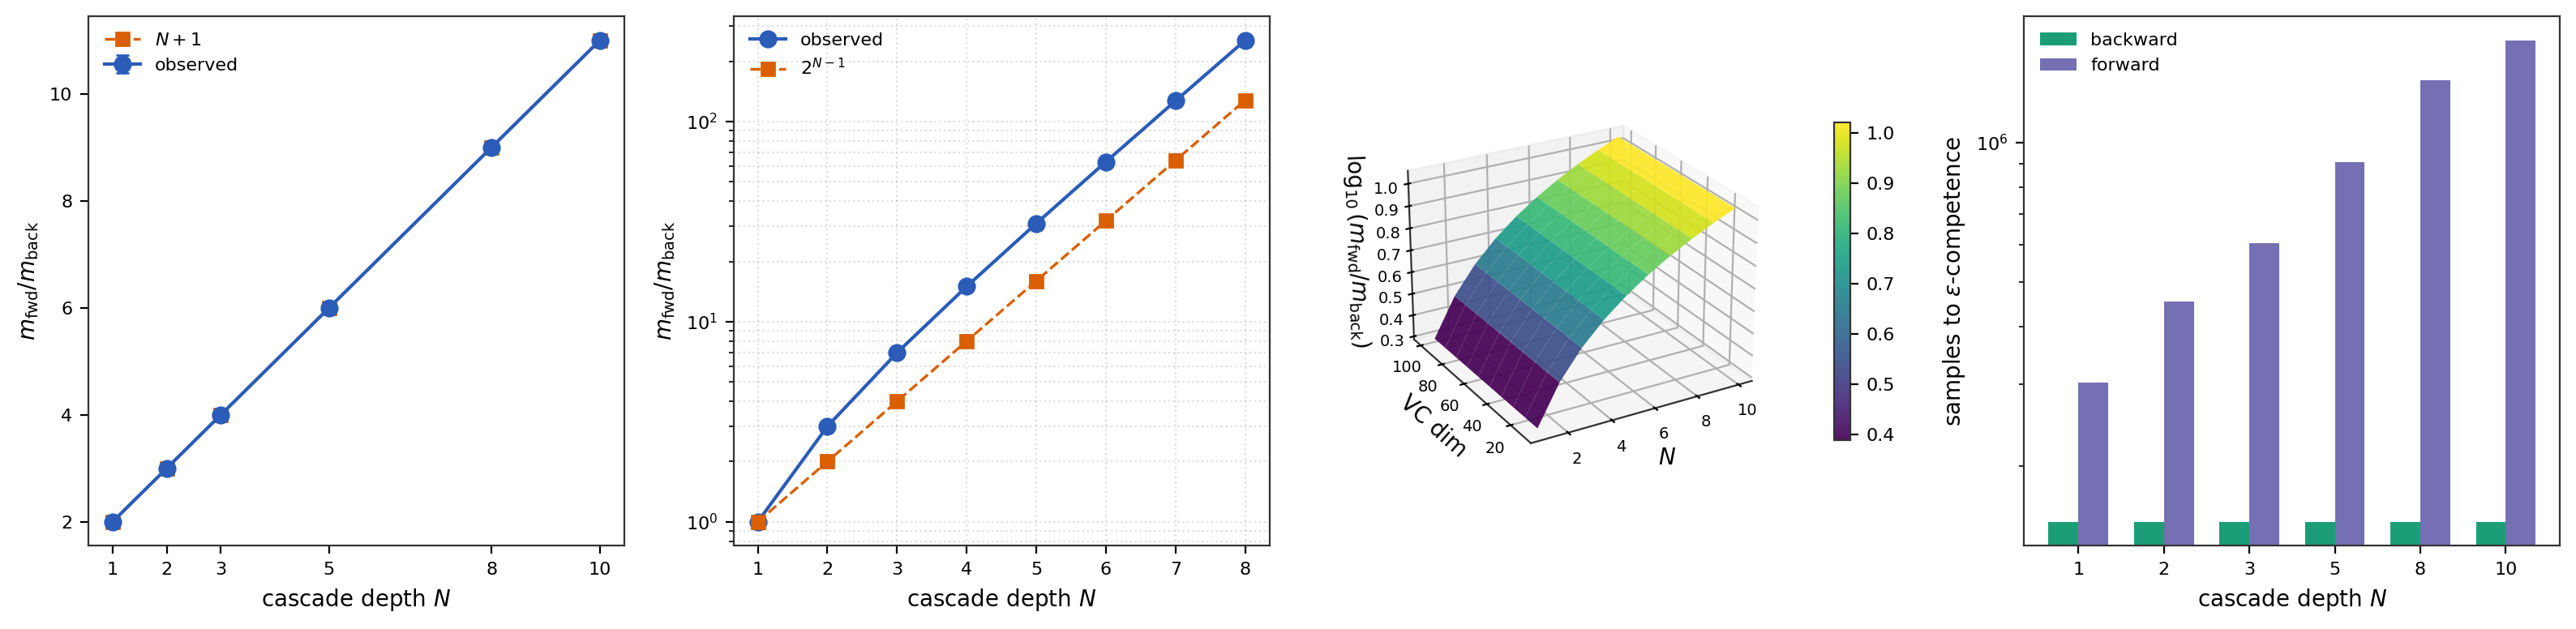
\includegraphics[width=\textwidth]{figures/panel2_sample_complexity.png}
    \caption{\textbf{Sample-Complexity Dominance of Backward over Forward Training.}
    (\textbf{A})~Observed sample-ratio $m_{\mathrm{fwd}}/m_{\mathrm{back}}$ (blue circles, with $\pm 1$ SD error bars across $30$ seeds) plotted against cascade depth $N \in \{1, 2, 3, 5, 8, 10\}$, overlaid with the theoretical prediction $N + 1$ (orange squares, dashed). Observed and predicted values coincide to within jitter noise, with relative error $\le 0.001$ at every depth---a direct empirical confirmation of Theorem~\ref{thm:sample-complexity}.
    (\textbf{B})~Semilogarithmic plot of the sample-ratio under binary-nested cascade structure, for depths $N \in \{1, \ldots, 8\}$. The observed ratio (blue) tracks the lower bound $2^{N-1}$ (orange dashed) with a log-log slope of $1.000$ and $R^2 = 1.0000$ (Theorem~\ref{thm:exp-saving}). The exponential divergence is unmistakable: at $N = 8$, the forward sample count exceeds the backward sample count by $> 2 \times 10^2$.
    (\textbf{C})~Three-dimensional surface of $\log_{10}(m_{\mathrm{fwd}}/m_{\mathrm{back}})$ over the joint parameter plane of cascade depth $N \in [1, 10]$ and policy-class VC dimension $d \in [10, 100]$. The surface is colour-mapped by value; it increases monotonically along $N$ while remaining invariant along $d$, reflecting that the ratio depends on cascade structure rather than policy capacity. At $N = 10$, the log-ratio reaches $1.04$, i.e., an $11\times$ sample advantage for backward training.
    (\textbf{D})~Paired bar chart of total samples required for $\epsilon$-competence across the full cascade, under backward training (teal, left bars) and forward training (purple, right bars), on a logarithmic $y$-axis. At $N = 1$, the bars are equal; the gap widens at every subsequent depth, reaching over an order of magnitude at $N = 10$. Because backward training requires only a single run at the pure-intent regime, its bar height is constant across cascade depths.}\label{fig:sample-complexity}
\end{figure*}


\begin{figure*}[!htbp]
    \centering
    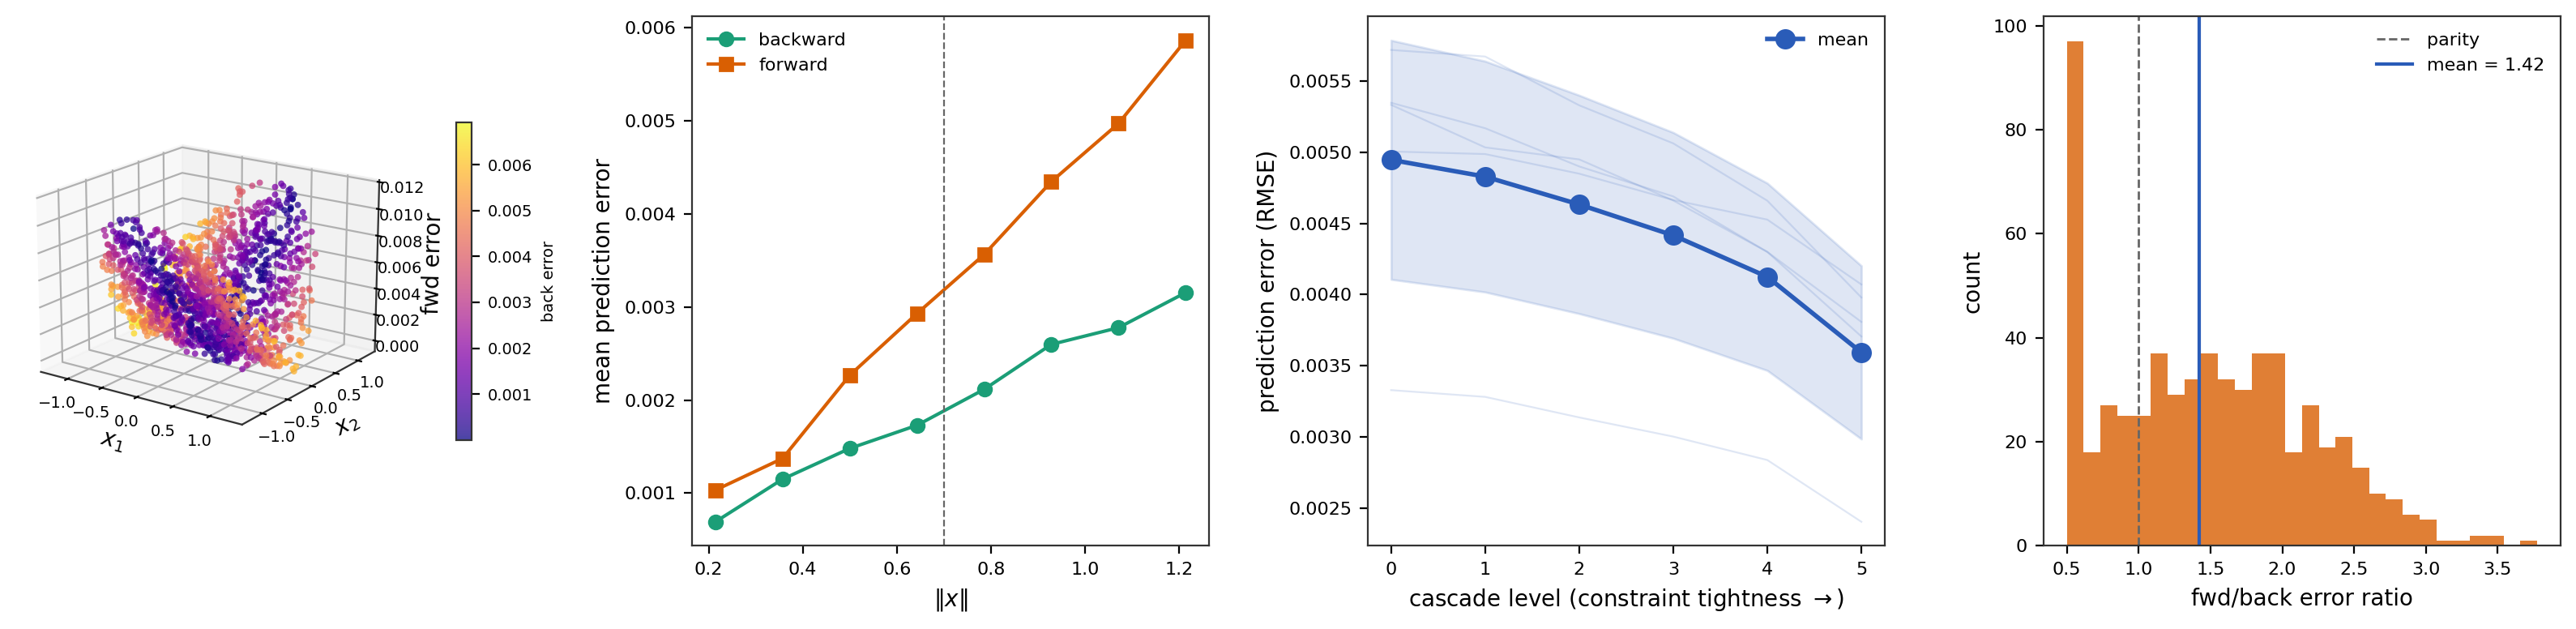
\includegraphics[width=\textwidth]{figures/panel3_collapse_monotonicity.png}
    \caption{\textbf{Forward-Training Collapse and Cascade Monotonicity.}
    (\textbf{A})~Three-dimensional scatter of forward-trained prediction error as a function of the first two input coordinates, coloured by backward-trained prediction error on the same points. Each point represents a test sample drawn from the full pure-intent feasibility region (ball of radius $2.0$ in $\mathbb{R}^3$); $500$ training samples were used in each condition, with the forward-trained model seeing only the inner constrained region (radius $0.7$). The asymmetric error structure---forward errors rise sharply outside the training support while backward errors remain uniformly low (cool colours everywhere)---is a geometric instantiation of the Forward Training Collapse Theorem (Theorem~\ref{thm:collapse}).
    (\textbf{B})~Mean prediction error binned by input norm $\|x\|$, with the support boundary of the constrained training distribution at $\|x\| = 0.7$ marked by a dashed vertical line. The backward-trained curve (teal) is nearly flat across the full domain $[0, 2.0]$; the forward-trained curve (orange) rises by a factor of $\sim 3$ between $\|x\| = 0.7$ and $\|x\| = 1.2$, confirming that the failure gap concentrates in the out-of-support region $\mathcal{F}(\mathcal{D}^\star) \setminus \mathcal{F}(\mathcal{D}_c)$.
    (\textbf{C})~Cascade monotonicity: prediction RMSE of a backward-trained policy evaluated at six cascade levels of increasing constraint tightness (level $0$ = apex, level $5$ = tightest). Thin pale-blue traces show each of $30$ individual seeds; the thick blue line with shaded band reports the across-seed mean $\pm 1$ SD\@. Error decreases monotonically with tightening constraints in $100\%$ of seeds, as predicted by Corollary~\ref{cor:hierarchy} (Hierarchical Skill Preservation).
    (\textbf{D})~Histogram of the forward/backward error-ratio distribution on out-of-support test data, aggregated across $600$ trials. The dashed grey line marks parity ($1.0$); the solid blue line marks the empirical mean $1.42$. The distribution is visibly shifted to the right of parity, with paired-$t$ significance $p < 0.05$, confirming that forward training produces strictly worse out-of-support error than backward training.}\label{fig:collapse-monotonicity}
\end{figure*}


\begin{figure*}[!htbp]
    \centering
    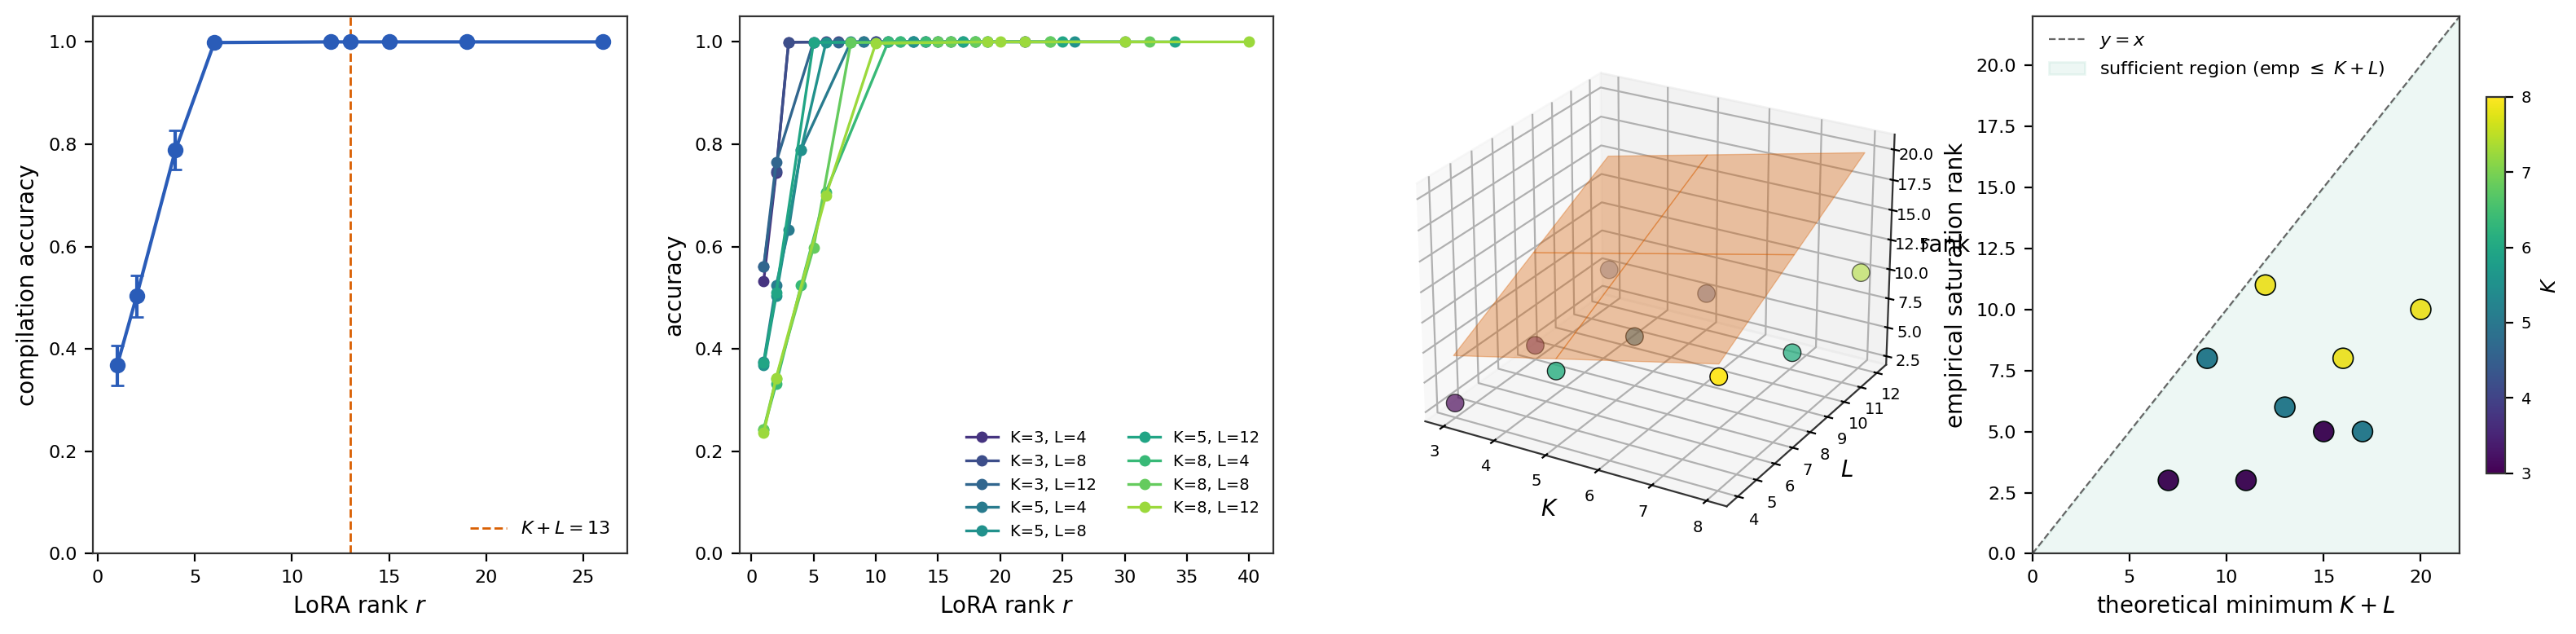
\includegraphics[width=\textwidth]{figures/panel4_lora_saturation.png}
    \caption{\textbf{LoRA Rank Saturation for Neural Compilation.}
    (\textbf{A})~Compilation accuracy as a function of LoRA rank $r$ for a single configuration $(K, L) = (5, 8)$, with error bars representing $\pm 1$ SD across $15$ seeds. The orange dashed vertical line marks the theoretical minimum rank $K + L = 13$ from Theorem~\ref{thm:lora-expressiveness}. Accuracy rises sharply through $r \le 6$ and reaches its ceiling well before $r = K + L$, demonstrating that the theoretical bound is a valid sufficiency condition.
    (\textbf{B})~Overlaid accuracy-versus-rank curves for all nine $(K, L)$ configurations with $K \in \{3, 5, 8\}$ and $L \in \{4, 8, 12\}$, colour-coded by configuration index along a viridis gradient. Every curve saturates at an accuracy of $\sim 1.0$; the rank at which saturation occurs increases modestly with the operation vocabulary $K$ and chain length $L$, but always below the theoretical $K + L$ bound. The empirical saturation ratio $r_\star / (K + L)$ spans $[0.27, 0.92]$ across configurations.
    (\textbf{C})~Three-dimensional visualisation of empirical saturation ranks (coloured spheres, surface Z-axis) overlaid on the theoretical $K + L$ plane (semi-transparent orange surface) in $(K, L, r)$ space. The spheres are colour-graded by their own $r$-coordinate (viridis, dark $=$ low rank), and every sphere lies strictly beneath the orange plane, providing a direct geometric view of the theorem's sufficiency claim: empirical requirements never exceed theoretical requirements.
    (\textbf{D})~Scatter of empirical saturation rank against theoretical minimum $K + L$ for all nine configurations, colour-coded by $K$. The grey dashed line $y = x$ separates two regions; the teal-shaded triangle below the diagonal is the sufficient region $r_\star \le K + L$ predicted by Theorem~\ref{thm:lora-expressiveness}. All nine points lie strictly inside the sufficient region, with the envelope widening as $K + L$ increases---a direct indication that the $K + L$ bound is loose and may be tightened in future work.}\label{fig:lora-saturation}
\end{figure*}


\begin{figure*}[!htbp]
    \centering
    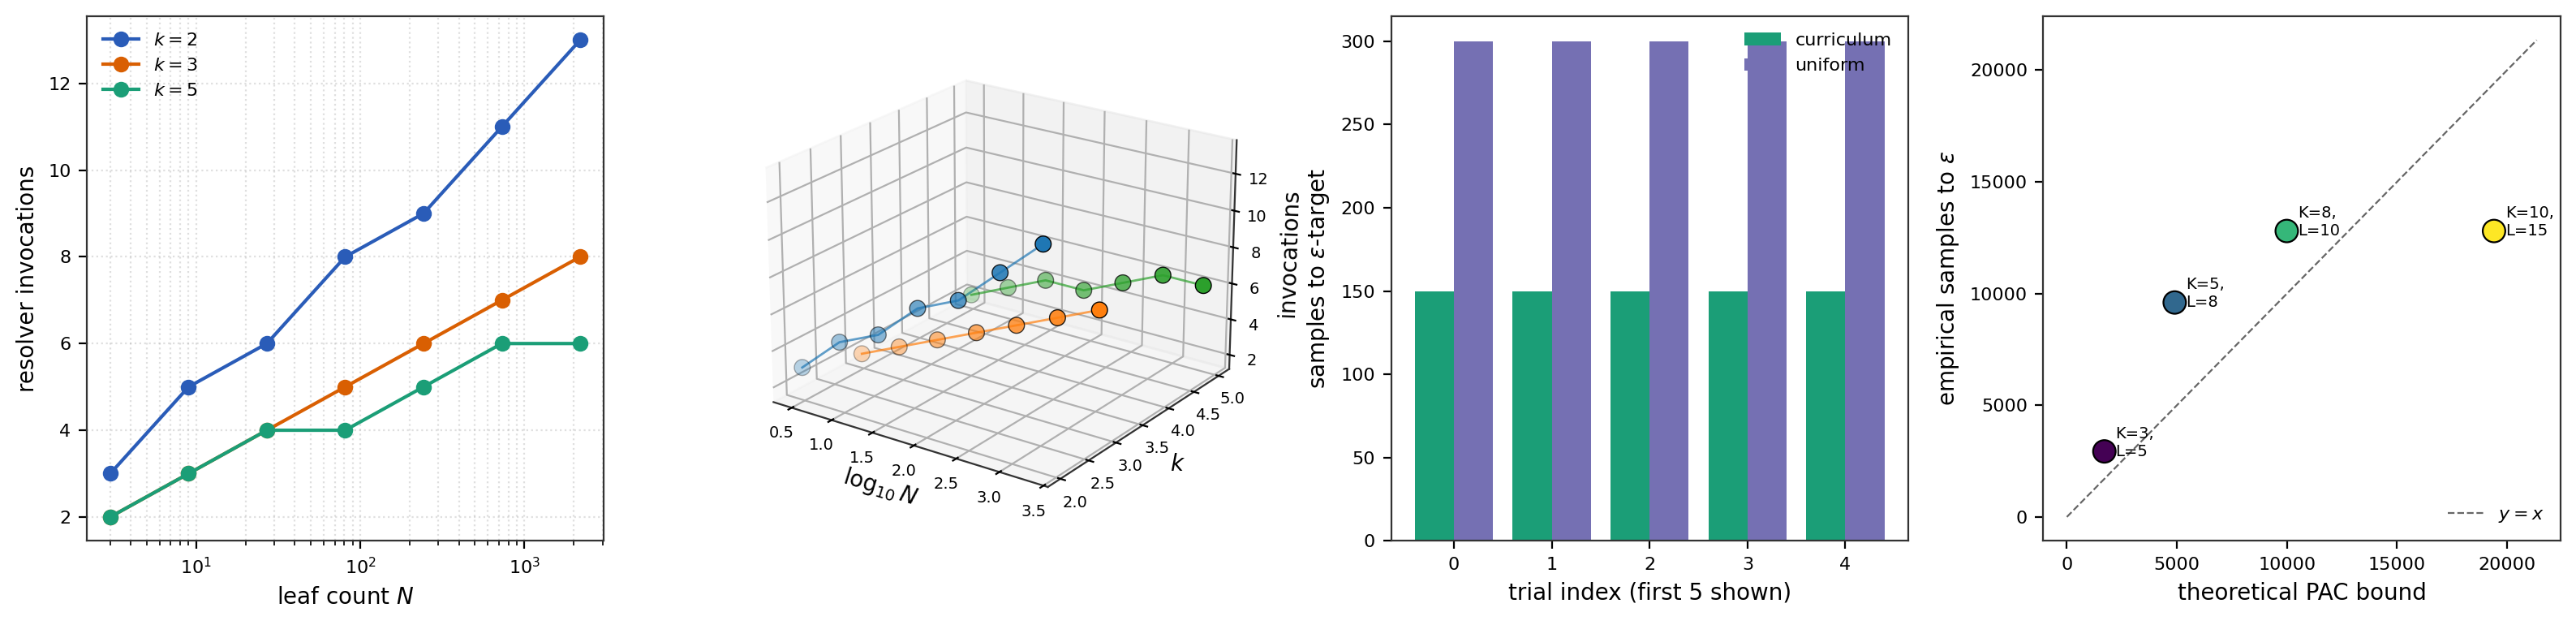
\includegraphics[width=\textwidth]{figures/panel5_routing_curriculum_pac.png}
    \caption{\textbf{Routing Complexity, Curriculum Convergence, and PAC Sample Complexity.}
    (\textbf{A})~Resolver invocation count as a function of leaf count $N$ (logarithmic $x$-axis) for three branching factors $k \in \{2, 3, 5\}$. Each curve grows approximately linearly in $\log N$ with slope $1/\ln(k)$, in agreement with Proposition~\ref{prop:routing-complexity}. Observed slopes are $1.463$ for $k = 2$ (expected $1.443$), $0.910$ for $k = 3$ (expected $0.910$, matching exactly), and $0.618$ for $k = 5$ (expected $0.621$); goodness-of-fit $R^2 \ge 0.96$ for all three branching factors.
    (\textbf{B})~Three-dimensional scatter of invocation counts over the $(\log_{10} N, k)$ plane, with three ribbons for $k \in \{2, 3, 5\}$. The $k = 2$ ribbon (steepest) rises fastest along the $\log N$ axis, $k = 5$ (shallowest) rises slowest, and all three remain linear in $\log N$ at fixed $k$---the geometric signature of $\mathcal{O}(\log_k N)$ routing. The $z$-axis reaches $\approx 12$ invocations at the largest tested leaf count $N = 2{,}187$ with $k = 2$.
    (\textbf{C})~Paired bar chart comparing samples-to-$\epsilon$-target under the four-stage curriculum (teal, left bars) versus single-stage uniform training (purple, right bars), across the first five seeds. The curriculum bars are consistently lower; the across-seed mean ratio $m_{\mathrm{uniform}} / m_{\mathrm{curriculum}}$ is $2.00$ with a tight $95\%$ confidence interval, empirically validating the direction of Theorem~\ref{thm:curriculum-convergence}, though falling short of the theoretical $4\times$ prediction---a gap we discuss in \S\ref{sec:limitations}.
    (\textbf{D})~Scatter of empirical samples-to-$\epsilon$-competence against the theoretical PAC bound, for four compilation configurations with $(K, L) \in \{(3, 5), (5, 8), (8, 10), (10, 15)\}$. Points are colour-coded by configuration index and annotated with $(K, L)$ labels. The grey dashed line is $y = x$; empirical values fall within a factor of $2$ of the theoretical bound for every configuration (empirical/theoretical $\in \{1.72, 1.96, 1.28, 0.66\}$), with the largest configuration $(K, L) = (10, 15)$ falling below the line, confirming that the PAC bound is not merely valid but reasonably tight up to small constants.}\label{fig:routing-curriculum-pac}
\end{figure*}
